\documentclass{article}
\input{preamble}

\usepackage{tikz}
\usetikzlibrary{positioning,arrows.meta}

\usepackage{color, soul}
% \soulregister{\cite}{1}

\usepackage{pdflscape}
\usepackage{booktabs}
\usepackage{longtable}
\usepackage{array}

\usepackage[
   backend=biber,
   sorting=none,
   sortcites=true,
]{biblatex}
\addbibresource{references.bib}

\begin{document}

\section{Definitions}
\textbf{Reinforcement learning}: learning paradigm where agent interacts at dicrete time steps $t=0,1,\dots,k$. At step $t$, the agent observes $s_t\in\calS$, acts with $a_t\in\calA$, receives reward $r_{t+1}\in\bbR$, and transitions to $s_{t+1}\in\calS$.
  \BI{
    \item Optionally, agent can receive $o_t\in\calO$; but the state can be modelled as a sequence of observations.
  }

  \textbf{Markov Decision Process}: A tuple $M=(\calS, \calA, P, r, \gamma)$ corresponding to the state space, action space, environment transition $P(s_{t+1}\mid s_t,a_t)$, reward function $r(s_t,a_t)$, discount factor $\gamma$.
  \BI{
    \item Implies no need for history of states. 
  }

  \textbf{Policy}: A distribution over actions conditioned on states $\pi(a\mid s)$ for all $a\in\calA$.
  \BI{
    \item The policy is \textbf{stationary} in that the mapping from states to actions does not change. 
  }

  \textbf{Rewards}: Provided by the environment to encourage goal-seeking behavior: $r(s,a)=\E{R_{t+1}\mid S_t,A_t}$. 

  \textbf{Return}: Reward aggregate over time. Defined as
  \BE{
    G_t=R_{t+1}+\cdots+R_T
  }
  for \textbf{episodic tasks}, or
  \BE{
    G_t=\sum_{k=0} \gamma^t R_{t+k+1}
  }
  for \textbf{continuing tasks}. 

  \textbf{Optimal policy}: The goal of RL is to determine
  \BE{
    \pi^*:=\argmax_{\pi\in\Pi} \Ep{\tau\sim P_\pi(\cdot)}{\sum_{t=0}^T r(s_t,a_t)}
  }

  \textbf{Occupancy Distribution}: The amount of time an agent spends in a (state, action) pair:
  \BE{
    d_\pi(s,a):=\sum_{t=0}^{T-1} P_\pi^t(s,a)
  }
  where $P_\pi^t(s,a)$ is the probability at time $t$ the agent is at $(s,a)$ when following policy $\pi$. 

  \textbf{State-value function}: The expected return from the state $s$ following $\pi$:
  \BE{
    v_\pi(s):=\Ec{G_t}{s_t=s}.
  }

  \textbf{Action-value function}: The expected return from the state $s$ taking some action $a$ following $\pi$:
  \BE{
    q_\pi(s,a):=\Ec{G_t}{s_t=s,a_t=a}.
  }

  \textbf{Optimal state/action-value function}: Defined as $v^*(s):=v_{\pi^*}(s)$ and $q^*(s,a):=q_{\pi^*}(s,a)$. 

  \textbf{Policy performance}: Expected return of a policy:
  \BE{
    J(\pi)=\E{\sum_{t=0}^\infty \gamma^t r(s_t,a_t)}=\Ep{s_0\sim \rho_0}{v_\pi(s_0)}.
  }

  \textbf{Prediction Problem}: Given an MDP and policy, determine the state and action value functions. 

  \textbf{Optimal Control}: Given an MDP, find $\pi^*$.

  Given $v^*$ for a discrete action-space, we can derive $\pi^*$ via
  \BE{
    \pi^*(a\mid s)=\argmax_{a\in\calA} \sum_{s',r}P(s',r\mid s,a)(r+\gamma v^*(s')).
  }

\section{Value-Based Methods}

  Three cases for value-based methods: finite with known rewards and dynamics, finite with unknown rewards and dynamics, and infinite. 

\subsection{Tabular Methods}

  \hl{\textbf{Bellman Expectation Equations (value form)}}: 
  \BE{
    v_\pi(s)=\sum_{a} \pi(a\mid s)\bbb{r(s,a)+\sum_{s'} P(s'\mid s,a)v_\pi(s')}
  }
  \textit{Proof}:
  \BA{
    v_\pi(s)
    &=\Ec{G_t}{s_t=s} \\
    &=\Ec{R_{t+1}+\gamma G_{t+1}}{s_t=s} \\
    &=\Ec{R_{t+1}}{s_t=s}+\gamma\Ec{G_{t+1}}{s_t=s} \\
    &=\sum_{a} \pi(a\mid s)r(s,a)+\gamma\sum_{a} \pi(a\mid s)\Ec{G_{t+1}}{s_t=s,a_t=a} \\
    &=\sum_{a} \pi(a\mid s)r(s,a)+\gamma\sum_{a} \pi(a\mid s)\sum_{s'} P(s'\mid s,a) v_\pi(s') \\
    &=\sum_{a} \pi(a\mid s)\bbb{r(s,a)+\sum_{s'} P(s'\mid s,a)v_\pi(s')}
  }

  \hl{\textbf{Bellman Expectation Equations (action form)}}:
  \BE{
    q_\pi(s)=r(s,a)+\sum_{s'} \bbb{P(s'\mid s,a) \sum_{a'} \pi(a'\mid s')q_\pi(s',a')}
  }
  \textit{Proof}:
  \BA{
    q_\pi(s)
    &=\Ec{G_t}{s_t=s,a_t=a} \\
    &=r(s,a)+\gamma\Ec{G_{t+1}}{s_t=s,a_t=a} \\
    &=r(s,a)+\sum_{s'} P(s'\mid s,a)\Ec{G_{t+1}}{s_{t+1}=s'} \\
    &=r(s,a)+\sum_{s'} \bbb{P(s'\mid s,a) \sum_{a'} \pi(a'\mid s')q_\pi(s',a')}
  }

  \textbf{Relationship between $v_\pi$ and $q_\pi$}:
  \BE{
    v_\pi(s)=\sum_{a} \pi(a\mid s)q_\pi(s,a)
  }

  \textbf{Bellman Optimality Equation (value form)}:
  \BE{
    v^*(s)=\max_a r(s,a)+\gamma\sum_{s'} P(s'\mid s,a)v^*(s')
  }

  \textbf{Bellman Optimality Equation (action form)}:
  \BE{
    q^*(s,a)=r(s,a)+\gamma\sum_{s'} P(s'\mid s,a)\max_{a'} q^*(s',a')
  }

  \textbf{Relationship between $v^*$ and $q^*$}:
  \BE{
    v^*(s)=\max_a q^*(s,a)
  }

  \textbf{Solving Bellman Expectation Equations}: Value functions are a linear system of equations:
  \BA{
    v_\pi
    &=r^\pi_s+\gamma T_{s's}^\pi v_\pi \\
    &v_\pi\in\bbR^{\bab{\calS}\times 1} \\
    &r_s^\pi=\sum_a \pi(a\mid s)r(s,a)\in \bbR^{\bab{\calS}\times 1} \\
    &T^\pi_{s's}=\sum_a \pi(a\mid s)P(s'\mid s,a)\in\bbR^{\bab{\calS}\times\bab{\calS}}
  }
  This can be solved using matrix inversion $v_\pi=(I-\gamma T^\pi)^{-1}r^\pi$. 

  \textbf{Advantage}:
  \BE{
    A_\pi(s,a):=q_\pi(s,a)-v_\pi(s)
  }

  \textbf{Bellman Expectation Operator}: 
  \BE{
    (T_\pi v)(s)=\sum_a \pi(a\mid s)\bbb{r(s,a)+\gamma\sum_{s'} P(s'\mid s,a)v(s')}
  }

  \textbf{Bellman Optimality Operator}:
  \BE{
    (T^* v)(s)=\max_a r(s,a)+\gamma\sum_{s'} P(s'\mid s,a)v(s')
  }

  \hl{\textbf{Iterative Policy Evaluation}}: Iteratively applies the Bellman expectation operator to $v^*$. This eventually converges to $v^*$:
  \BE{
    v_{[k+1]}(s):=T_\pi v_{[k]}.
  }

  \textbf{Value Iteration}: Iteratively applies the Bellman optimality operator to $v^*$ until convergence:
  \BE{
    v_{[k+1]}(s):= T^* v_{[k]}.
  }

  \hl{\textbf{Policy Iteration}}: Run policy evaluation until convergence to compute $v_{\pi_k}$ (e.g. closed form, iterative policy evaluation, etc.). Then, recompute $\pi$ via
  \BE{
    \pi_k(a\mid s)=\argmax_a r(s,a)+\sum_{s'} P(s'\mid s,a)v_{\pi_{k-1}}(s')
  }
  \BI{
  \item Value iteration is a special case of policy iteration with a single policy evaluation at each step. Bellman optimality operators do not require a policy $\pi$, so computing this can be skipped. 
  }

  Limitations of tabular methods: computation required for all states, even ones that are unlikely. Not applicable to continuous state or action spaces.

\subsection{Model-Free Prediction}

  \hl{\textbf{Monte-Carlo Policy Evaluation}}: Learn $v_\pi(s)$ from episodes of experience under $\pi$:
  \BA{
    N(s_t)&\leftarrow N(s_t)+1 \\
    V(s_t)&\leftarrow V(s_t)+\frac{1}{N(s_t)} (G_t-V(s_t))
  }
  \BI{
    \item For non-stationary problems, track running means $V(s_t)\leftarrow V(s_t)+\alpha(G_t-V(s_t))$.  
    \item Update rule applies to both \textbf{first-visit MC} or \textbf{every-visit MC}.
    \item Monte-Carlo control uses the same algorithm for the action value function. 
  }

  \hl{\textbf{Monte-Carlo Control}}: An algorithm that alternates between Monte-Carlo policy evaluation and policy improvement. The most basic form of policy improvement is given by
  \BE{
    \pi(s)\leftarrow \argmax_a q(s,a).
  }
  \BI{
    \item MC control is \textbf{on-policy} because trajectories collected by the policy are used to improve it in the following step and then discarded. 
  }

  \textbf{Exploration Problem}: Policy needs to act suboptimally to explore all actions.

  \textbf{$\epsilon$-soft Policies}: The probability of an action $\pi(a\mid s)$ is $\epsilon/\bab{\calA(s)}$ for the non-optimal action or $(1-\epsilon)+\f{\epsilon}{\bab{\calA(s)}}$ otherwise. In Monte-Carlo policy evaluation, this is used to address the exploration problem.
  \BI{
    \item Disadvantage: The second-best action is ranked equally with the worst-possible action. 
  }

  \hl{\textbf{Temporal Difference Prediction}}: \textbf{TD(0)} bootstraps MC policy evaluation with current goal estimate after one step:
  \BE{
    V(s_t)\leftarrow V(s_t)+\alpha(R_{t+1}+\gamma V(s_{t+1})-V(s_t)). 
  }
  The term $R_{t+1}+\gamma V(s_{t+1})$ is called the \textbf{TD target}.
  \BI{
    \item Compared to MC policy iteration, TD has lower variance and is instantaneous (can be evaluated online, instead of waiting for $G_t$ to be computed after following the whole trajectory). 
  }

  \textbf{$n$-step TD Learning}: Uses goal $G_t^{(n)}$ defined as
  \BE{
    G_t^{(n)}:= R_{t+1}+\gamma R_{t+2}+\cdots+\gamma^{n-1} R_{t+n}+ \gamma^n V(s_{t+n})
  }
  \BI{
    \item TD(0)$\equiv$ $0$-step TD learning, MC control $\equiv$ $\infty$-step TD learning. In general, increasing $n$ leads to higher variance, lower bias. 
  }

  \hl{\textbf{SARSA}}: Uses action-valued TD learning:
  \BE{
    Q(s_t,a_t)\leftarrow Q(s_t,a_t)+\alpha(R_{t+1}+\gamma Q(s_{t+1},a_{t+1})-Q(s_t,a_t))
  }
  For each step, take action $a$ and observe new state $s'$ and reward $r$. Pick $a'$ from $s'$ from policy derived from $Q$ (e.g. $\epsilon$-greedy). \underline{SARSA is on-policy}. 

  \hl{\textbf{Q-Learning}} \cite{watkins1992q}: Performs greedy, off-policy TD learning:
  \BE{
    Q(s_t,a_t)\leftarrow Q(s_t,a_t)+\alpha(R_{t+1}+\gamma \max_a Q(s',a)-Q(s_t,a_t)).
  }
  \BI{
    \item SARSA is ``safe'' because it accounts for random steps, e.g. in tasks like cliff-walking. Q-learning is capable of taking risks because it assumes that the optimal policy is used for future steps.
    \item Reduces variance from SARSA, but introduces maximization bias. 
  }

  \textbf{Maximization Bias}: Consider $(s,a)$ s.t. $q^*(s,a)=0$ and $Q(s,a)>0$. Then, $Q(s,\argmax_a Q(s,a))>0$, but $q^*(s,\argmax_a q^*(s,a))=0$. This results from using the same $Q$ function to compute and evaluate the argmax. 

  \hl{\textbf{Double Q-Learning}}: Train two functions $Q_1,Q_2$. Perform $Q$-learning on different time steps and pick at reandom which function to update. Use $Q_2$ to compute the next state for $Q_1$ and vice versa:
  \BA{
    a^*&\leftarrow \argmax_a Q_1(s',a) \\
    Q_1(s_t,a_t)&\leftarrow Q(s_t,a_t)+\alpha(R_{t+1}+\gamma Q_2(s',a^*)-Q_1(s_t,a_t))
  }
  This works because it decouples selecting the best action from assigning a value to the best action. 

  \hl{\textbf{Expected SARSA}}: Uses an \textbf{expected TD target}: 
  \BE{
    r+\gamma\Ep{a\sim\pi(\cdot\mid s_{t+1})}{Q(s_{t+1},a)}=r+\gamma\sum_a \pi(a\mid s_{t+1}))Q(s_{t+1},a)
  }
  \BI{
    \item When using a greedy policy (not $\epsilon$-greedy), SARSA, Q-learning, and expected SARSA are equivalent.
    \item Reduces variance from SARSA.
  }

\subsection{Deep RL Methods}
  
  Function approximation: represent Q-values as a learned function parameterized by $\theta$. 

  \textbf{Neural representations of value functions}: Approximate $v_\pi$ and $q_\pi$ with $V_\theta(s_t)$ and $Q_\theta(s_t,a_t)$ where $\bab{\theta}<\bab{\calS}$. Goal is to find
  \BE{
    \argmin_\theta J(\theta)=\Ep{\pi}{(v_\pi(s)-V_\theta(s))^2}.
  }
  The corresponding gradient decent updates are
  \BE{
    \Delta \theta=-\f{1}{2} \alpha\nabla_\theta J(\theta)=\alpha \Ep{\pi}{(v_\pi(s)-V_\theta(s))\nabla_\theta V_\theta(s)}
  }
  where the \textbf{target} is $v_\pi(s)$.
  \BI{
    \item Target is return $G_t$ in MC policy iteration, $R_{t+1}+\gamma V_\theta(s_{t+1})$ in TD(0).
  }

  Loss function is similar for action value functions. For example, for TD estimation,
  \BE{
    \Delta\theta =-\alpha\nabla_\theta J(\theta)=\alpha(R_{t+1} + \gamma\max_a Q_\theta(s_{t+1},a)-Q_\theta(s_t,a_t)) \nabla_\theta Q_\theta (s_t,a_t)
  }

  \textbf{Deadly Triad}: Naive Q-Learning using a parameterized Q function and a least-squares objective
  \BE{
    \min_\theta \f{1}{2}\bpa{Q_\theta(s,a)-(r(s,a)+\gamma\max_{a'} Q_\theta(s',a'))}^2
  }
  is off-policy, uses function approximation, and bootstrapping, which makes convergence and efficient learning extremely difficult. 

  \hl{\textbf{Deep Q-Learning}} \cite{mnih2015human}: Introduces a \textbf{target network} $Q_{\theta^-}$ which is a copy of the \textbf{online network} $Q_\theta$ delayed by some amount which gives a stable estimation of the value function. Also uses an \textbf{experience replay buffer} that stores $(s,a,r,s')$ tuples from many trajectories and allows for data decorrelation and improved sample efficiency. The TD target is given by
  \BE{
    y^\text{DQN}=r+\gamma\max_{a'} Q_{\theta^-}(s',a').
  }
  \BI{
    \item In practice, this is implemented as a neural network $Q_\theta: \calS\to \bbR^{\bab{\calA}}$. 
  }

  \hl{\textbf{Double DQN}} \cite{van2016deep}: Deep Q-Learning using the online network to select the next action but using the target network to evaluate it:
  \BA{
    a^*&=\argmax_a Q_\theta(s',a') \\
    y^\text{Double-DQN}&=R_{t+1}+\gamma Q_{\theta^-}(s',a^*)
  }

  \hl{\textbf{Clipped Double DQN}} \cite{fujimoto2018addressing}: Use the minimum of target and online network to evaluate the Q function:
  \BE{
    y^\text{Clipped-Double-DQN}=R_{t+1}+\min_{Q\in\bbr{Q_\theta, Q_{\theta^-}}} Q(s',a^*).
  }

  \textbf{Prioritizing Replays \cite{schaul2016prioritized}}: Within the experience replay buffer, weight each experience by its ``surprise'' or DQN error:
  \BA{
    p_i&=r_i+\gamma\max_{a} Q_{\theta^-}(s'_i,a)-Q_{\theta}(s'_i,a) \\
    P(i)&=\f{p_i^\alpha}{\sum_k p_k^\alpha}.
  }
  \BI{
    \item $\alpha$ parameterizes how much the priority is used, with $\alpha=0$ being the uniform case. 
  }

  \textbf{Multistep Q-Learning}:
  \BE{
    I=(R^{(n)}_t+\gamma_t^{(n)}\max_{a'} Q_{\theta^-}(S_{t+n},a') - Q_\theta(s,a))^2.
  }

\section{Evolutionary Methods}

  \hl{\textbf{Policy optimization}}: policy optimization methods search over policy parameters without computing state or action values:
  \BE{
    \max_\theta U(\theta)=\Epc{\tau\sim\pi_\theta}{R(\tau)}{\pi_\theta,\mu_0(s_0)}.
  }

  \textbf{Univariate Gaussian Distribution}:
  \BE{
    \calN(y\mid \mu,\sigma^2)=\f{1}{\sqrt{2\pi\sigma^2}}\exp\bpa{\f{-(y-\mu)^2}{2\sigma^2}}.
  }

  \textbf{Multivariate Gaussian Distribution}:
  \BE{
    \calN(y\mid \mu,\Sigma)=\frac{1}{(2\pi)^{d/2}\bab{\Sigma}^{1/2}}\exp\bpa{-\f{1}{2} (y-\mu)^\top \Sigma^{-1}(y-\mu)}.
  }

  \hl{\textbf{Cross-entropy Method}}: Initialize $\mu_0\leftarrow 0$, $\Sigma_0\leftarrow I$. For each step, sample $\theta_i\in\calN(\mu,\sigma^2I)$ for $i=1,\dots,N$. For each, evaluate over $L$ trials and take top $\bcl{\rho N}$ $\theta_i$ by mean overall reward. Then, update via
  \BA{
    \mu_t&\leftarrow \f{1}{K}\sum_{i\in \varepsilon}\theta_i \\
    \Sigma_t&\leftarrow \f{1}{K}\sum_{i\in\varepsilon}(\theta_i-\mu_{t+1})(\theta_i-\mu_{t+1})^\top.
  }
  \BI{
    \item Optionally, add smoothing $\mu_t\leftarrow (1-\alpha)\mu_t+\alpha \mu_{t-1}$, $\Sigma_t\leftarrow (1-\alpha)\Sigma_t+\alpha \Sigma_{t-1}$. 
  }

  \hl{\textbf{Natural Evolutionary Strategy}}: Maximize
  \BE{
    \max_\mu \Ep{\theta\sim P_\mu(\theta)} {F(\theta)}
  }
  where $P_\mu(\theta)=\calN(\mu,\sigma^2I)$ ($\sigma^2$ is a constant hyperparameter) and $F(\theta)=\Ep{\tau\sim\pi_0,s_0\sim\mu_0(s)}{R(\tau)}$. The corresponding gradient update is
  \BA{
    \nabla_\mu \Ep{\theta\sim P_\mu(\theta)} {F(\theta)}
    &=\nabla_\mu \int P_\mu(\theta)F(\theta)\d \theta \\
    &=\int P_\mu(\theta)\cdot\f{\nabla_\mu P_\mu(\theta)}{P_\mu(\theta)}F(\theta)\d \theta \\
    &=\int P_\mu(\theta)\cdot\nabla_\mu \log P_\mu(\theta) F(\theta)\d \theta \\
    &=\Ep{\theta\sim P_\mu(\theta)}{\nabla_\mu \log P_\mu(\theta) F(\theta)} \\
    &\approx \f{1}{N} \sum_{i=1}^N \nabla_\mu \log P_\mu(\theta) \vert_{\theta=\theta_i} F(\theta_i)
  }
  where $\theta_i\sim P_\mu(\theta)$. We also have that
  \BE{
    \nabla_\mu \log P_\mu(\theta)=\nabla_\mu -\f{\bnm{\theta-\mu}^2}{2\sigma^2}=\f{\theta-\mu}{\sigma^2}.
  }
  We can express $\theta=\mu+\sigma\epsilon$ for $\epsilon\sim\calN(0,1)$, so the gradient becomes
  \BA{
    \nabla_\mu \Ep{\theta\sim P_\mu(\theta)}{F(\theta)}\approx \f{1}{N\sigma} \sum_{i=1}^N \epsilon_i F(\mu+\sigma\epsilon_i).
  }

  \textbf{Distributed Evolution}: Server broadcasts seeds $s_1,\dots,s_k$; each core $i\in[k]$ computes $\epsilon_j$ from seed $s_i$ and broadcasts aggregate result back to the server.

\section{Policy-Gradient Methods}

  \hl{\textbf{Policy Optimization}}: For some objective function $U(\theta)$, sample trajectories $\tau_i=\bbr{s_t^i,a_t^i}_{t=0}^T$ by deploying $\pi_\theta$ and then update $\theta\leftarrow \theta+\alpha\nabla_\theta U(\theta)$. 

  \textbf{Policy Objectives}: The parameterization of the network depends on the type of task:
  \BI{
  \item Deterministic discrete/continuous: $a=\pi_\theta(s)$
  \item Stochastic continuous: $a\sim \calN(\mu_\theta(s),\sigma^2_\theta(s))$
  \item Stochastic discrete: $a\sim \mathrm{softmax}(\cdot)$.
  }
  In general, a reasonable policy objective is
  \BA{
    \max_\theta U(\theta)&=\Ep{\tau\sim P(\tau;\theta)}{R(\tau)}=\sum_{\tau} P(\tau;\theta)R(\tau) \\
    P(\tau;\theta)&=\rho_0(s_0)\prod_{t=0}^H \underbrace{P(s_{t+1}\mid a_t,s_t)}_\text{dynamics}\underbrace{\pi_\theta(a_t\mid s_t)}_\text{policy}
  }
  In this form, backpropogation is not directly applicable because to get $\nabla_\theta P(\tau;\theta)$ requires knowing the dynamics of the environment.
  \BI{
  \item The gradiant can be numerically approximated, but this is not feasible for high-dimensional parameter spaces:
    \BE{
      \pypx{U(\theta)}{\theta_k}\approx\f{U(\theta+\epsilon u_k)-U(\theta-\epsilon u_k)}{2\epsilon}.
    }
  }

\subsection{REINFORCE and Actor-Critic Algorithms}

  \textbf{General Policy Score}: Consider the following expression for $P(\cdot)$ continuous, differentiable, and easy to sample:
  \BA{
    \nabla_\theta \Ep{x\sim P_\theta(x)}{f(x)}
    &=\nabla_\theta \int P_\theta(x)f(x) \d x \\
    &=\int \nabla_\theta P_\theta(x)f(x) \d x \\
    &=\int \f{\nabla_\theta P_\theta(x)}{P_\theta(x)} P_\theta(x)f(x)\d x \\
    &=\int P_\theta(x)\cdot \nabla_\theta \log P_\theta(x)f(x)\d x \\
    &=\Ep{x\sim P_\theta(x)}{\nabla_\theta \log P_\theta(x)f(x)} \\
    &\approx \f{1}{N}\sum_{i=1}^N \nabla_\theta \log P_\theta(x^{(i)})f(x^{(i)}).
  }
  This form is easier to work with because one only needs to evaluate $\nabla_\theta \log P_\theta(x)$ for $x$ sampled from $P_\theta(x)$.
  \BI{
    \item Note that we still need trajectories $\tau^{(i)}\sim P_\theta$ to remain on-policy.
    \item This expression can be interpreted as a weighted sum pulling the gradient towards directions with higher rewards. 
  }

  \textbf{Policy Scores for Gaussian and Softmax Policies}: We have that
  \BA{
    \nabla_\theta \log P_\theta(\tau)
    &=\nabla_\theta \log \bpa{\prod_{t=0}^T P(s_{t+1}^{(i)}\mid s_t^{(i)},a_t^{(i)})\pi_\theta(a_t^{(i)}\mid s_t^{(i)})} \\
    &=\nabla_\theta \sum_{t=0}^T \log\pi_\theta(a_t^{(i)}\mid s_t^{(i)}) \\
    &=\sum_{t=0}^T \nabla_\theta \log\pi_\theta(a_t^{(i)}\mid s_t^{(i)})
  }
  \BI{
    \item For Gaussian policies,
      \BE{
        \nabla_\theta \log\pi_\theta(a\mid s)\propto (\Sigma^{-1}(a-\mu_\theta(s)))^\top\pypx{(\mu_1,\dots,\mu_m)}{(\theta_1,\dots,\theta_n)}
      }
    \item For softmax policies,
      \BE{
        \nabla_\theta \log\pi_\theta(a\mid s)=\nabla_\theta h_\theta(s,a)-\sum_{a'} \pi_\theta(a'\mid s)\nabla_\theta h_\theta(s,a'),
      }
      where $\pi_\theta(a\mid s)=\exp(h_\theta(s,a))/\sum_{a'}(\cdot)$. 
  }

  \textbf{Cold-Start Problem}: For trajectories with $0$ reward, policy just randomly explores. 

  \hl{\textbf{REINFORCE Algorithm}} \cite{williams1992simple}: Combining the two previous derivations with reward function $f(x)=G_t$, we get
  \BE{
    \hat{g}=\f{1}{N}\sum_{i=1}^N \sum_{t=1}^T \nabla_\theta \log\pi_\theta(a_t^{(i)}\mid s_t^{(i)})G^{(i)}_t
  }
  \BE{
    \theta_{t+1}\leftarrow \theta_t +\alpha\gamma^t G_t\f{\nabla_\theta \pi_\theta(a_t\mid s_t)}{\pi_\theta(a_t\mid s_t)}
  }
  Compared with the MC policy iteration method, REINFORCE samples over parameter space instead of action space. 

  \textbf{State-Dependent Baseline}: A state-based baseline may be subtracted from the REINFORCE gradient without changing the gradient:
  \BE{
    \sum_{t=0}^H (G_t-b(s_t))\nabla_\theta \log \pi_\theta(a_t\mid s_t)
  }
  since $\Ep{a\sim\pi_\theta(\cdot\mid s)}{\nabla_\theta \log \pi_\theta(a\mid s)}=0$. Setting $b(s_t)=v_\pi(s)$ reduces variance:
  \BE{
    \Var(\hat{g})=\mathrm{tr}\;\E{(\hat{g}-\E{\hat{g}})(\hat{g}-\E{\hat{g}})^\top}=\sum_{i=1}^n \E{(\hat{g}_k-\E{\hat{g}_k})^2}.
  }
  \BI{
  \item Motivation: We care about the advantage of an action conditioned on a state, not only when it has high returns:
    \BE{
      G_t-v_\pi(s_t)\approx q_\pi(s_t,a_t)-v_\pi(s_t)=A_\pi(s_t,a_t).
    }
  }

  \hl{\textbf{Actor-Critic Algorithm}} \cite{sutton1999policy}: Let $V^\pi_\phi(s_t)$ parameterized by $\phi$ approximate $v_\pi(s_t)$ from trajectories derived from $\pi$. The approximate value function can be computed at each step using standard value-based approaches:
  \BI{
  \item Monte-Carlo:
    \BE{
      \phi\leftarrow \argmin_\phi \f{1}{N}\sum_{i=1}^N \sum_{t=0}^T \bpa{V_\phi^\pi(s_t^{(i)}-G_t^{(i)})}^2.
    }
  \item TD(0):
    \BE{
      \phi\leftarrow \argmin_\phi \sum_{(s,a,r,s')}\bnm{r+\gamma V_\phi^\pi(s')-V^\pi_\phi(s)}_2^2
    }
  }
  The pseudocode for actor-critic:
  \BN{
  \item Sample $\tau_i=\bbr{s_t^{(i)},a_t^{(i)}}_{t=1}^T$ by deploying policy $\pi_\theta$.
  \item Update $\phi$ by fitting $V_\phi^\pi$ with MC/TD(0) methods.
  \item Compute advantages $A^\pi(s_t^{(i)},a_t^{(i)})=G_t^{(i)}-V_\phi^\pi(s_t^{(i)})$.
  \item Update $\theta$ via
    \BA{
      \nabla_\theta U(\theta)&\approx \f{1}{N}\sum_{i=1}^N \sum_{t=1}^T \nabla_\theta \log\pi_\theta(a_t^{(i)}\mid s_t^{(i)}) A_\pi(s_t^{(i)},a_t^{(i)}) \\
      \theta&\leftarrow \theta+\alpha\nabla_\theta U(\theta).
    }
  }

  \hl{\textbf{Advantage Actor-Critic (A2C)}} \cite{mnih2016asynchronous}: We can express $A_\pi(s_t^{(i)},a_t^{(i)})=Q_\phi^\pi(s_t^{(i)},a_t^{(i)})-V_\phi^\pi(s_t^{(i)})$ where $Q_\phi^\pi(s_t^{(i)},a_t^{(i)})=R(s_t^{(i)},a_t^{(i)})+\gamma V_\phi^\pi(s_{t+1}^{(i)})$. 

  \textbf{High Data Correlation}: Trajectory samples taken in actor-critic algorithms are high correlated, but stochastic gradient requires uncorrelated, uniformly sampled data. Furthermore, actor-critic algorithms are required to be on-policy (so experience buffer does not work). This can be solved in practice by running many RL environments in parallel. 

  \textbf{Entropy Regularization}: The \textbf{Shannon entropy} of a state-conditioned policy is given by
  \BE{
    \calH(\pi(\cdot\mid s))=-\sum_a \pi(a\mid s)\log \pi(a\mid s)=-\Ep{a\sim \pi(\cdot\mid s)}{\log \pi(a\mid s)}.
  }
  We add this term to the actor loss:
  \BE{
    U(\theta)=\Ep{\tau\sim P(\tau;\theta)}{R(\tau)-\beta \calH(\pi_\theta(\cdot\mid s_t))}.
  }
  This can be differentiated via
  \BE{
    \nabla_\theta \calH(\pi_\theta(a\mid s))=-\Ep{a\sim \pi_\theta(\cdot\mid s)}{\nabla_\theta \log \pi_\theta(a\mid s)(\log \pi_\theta(a\mid s)+1)}.
  }

  \textbf{Update-to-Data (UTD) Ratio}: The update-to-data ratio is defined as the number of gradient update divided by the number of new environment transitions. A high UTD leads to being too off-policy and makes it unable to escape local minimums, whereas a low UTD is data inefficient. 

\subsection{PPO}

  \hl{\textbf{Performance Difference Lemma}}: 
  \BE{
    J(\pi')-J(\pi)=\Ep{s\sim d^{\pi'},a\sim\pi'(\cdot\mid s)}{A_\pi(s,a)}.
  }
  \textit{Proof}: We have that
  \BA{
    \Ep{a\sim\pi'}{A_\pi(s,a)}
    &=\Ep{a\sim\pi'}{q_\pi(s,a)-v_\pi(s)} \\
    &=\Ep{a\sim\pi'}{q_\pi(s,a)} -v_\pi(s) \\
    &=\Ep{a\sim\pi'}{r(s,a)}+ \gamma\Ep{a\sim\pi',s'\sim P(\cdot\mid s,a)}{v_\pi(s',a)}-v_\pi(s).
  }
  For fixed $(s_t,a_t)$ from $\pi'$ with $s_0\sim \rho_0$, we have
  \BA{
    \Ep{\pi'}{A_\pi(s_t,a_t)}&=\Ep{\pi'}{r_t}+\gamma \Ep{\pi'}{v_\pi(s_{t+1})}-\Ep{\pi'}{v_\pi(s_t)} \\
    \sum_{t=0}^\infty \gamma^t\Ep{\pi'}{A_\pi(s_t,a_t)}
    &=\sum_{t=0}^\infty \gamma^t\bpa{\Ep{\pi'}{r_t}+\gamma \Ep{\pi'}{v_\pi(s_{t+1})}-\Ep{\pi'}{v_\pi(s_t)}} \\
    &=\bpa{\sum_{t=0}^\infty \gamma^t \Ep{\pi'}{r^t}}-\Ep{s_0\sim\rho_0}{v_\pi(s_0)} \\
    &=J(\pi')-J(\pi).
  }
  By definition, we have
  \BE{
    \Ep{s\sim d^{\pi'},a\sim\pi'(\cdot\mid s)}{A_\pi(s,a)}=\sum_{t=0}^\infty \gamma^t\Ep{\pi'}{A_\pi(s_t,a_t)},
  }
  concluding the proof. 

  \textbf{Importance Sampling}: Consider the problem of computing $\Ep{z\sim p}{f(z)}=\int f(z)p(z)\d z$ but $p(z)$ cannot be sampled directly. Instead, a \textbf{proposal distribution} $q(z)$ can be sampled from. We have that
  \BE{
    \Ep{z\sim p}{f(z)}=\Ep{z\sim q}{\f{p(z)}{q(z)} f(z)}\approx \f{1}{N}\sum_{i=1}^N \underbrace{\f{p(z^{(i)})}{q(z^{(i)})}}_\text{importance weight} f(z^{(i)})
  }

  \textbf{Importance-Weighted Policy Gradients}: Policy optimization reduces to 
  \BE{
    \max_{\pi'} J(\pi')=\max_{\pi'} J(\pi')-J(\pi)=\max_{\pi'} \Eb_{s\sim d^{\pi'}}\Ep{a\sim\pi'(\cdot\mid s)}{A_\pi(s,a)}
  }
  We approximate $d^\pi(s)\approx d^{\pi'}(s)$ so that we can sample states from the existing policy $\pi$ and apply the distribution shift correction from $\pi'(\cdot\mid s)$ to $\pi(\cdot\mid s)$:
  \BE{
    \Eb_{s\sim d^{\pi'}}\Ep{a\sim\pi'(\cdot\mid s)}{A_\pi(s,a)}
    =\Eb_{s\sim d^{\pi'}}\Ep{a\sim\pi(\cdot\mid s)}{\f{\pi'(a\mid s)}{\pi(a\mid s)}{A_\pi(s,a)}}
    \approx\Eb_{s\sim d^{\pi}}\Ep{a\sim\pi(\cdot\mid s)}{\f{\pi'(a\mid s)}{\pi(a\mid s)}{A_\pi(s,a)}} 
  }
  We have that
  \BE{
    \nabla_{\theta'}\Eb_{s\sim d^{\pi}}\Ep{a\sim\pi(\cdot\mid s)}{\f{\pi'(a\mid s)}{\pi(a\mid s)}{A_\pi(s,a)}}=\Eb_{s\sim d^{\pi}}\Ep{a\sim\pi(\cdot\mid s)}{\nabla_{\theta'}\log \pi'(a\mid s)\f{\pi'(a\mid s)}{\pi(a\mid s)}{A_\pi(s,a)}}
  }
  (recall that $\nabla_\theta \log\pi(a\mid s)$ has a closed-form solution for Gaussian and softmax policies). To account for the approximation, we add a penalty term to the loss to make it a \textbf{constrained maximization} problem:
  \BE{
    \max_{\pi'} (\cdot) - \alpha\Ep{s}{\calD_\text{KL}(\pi'(\cdot\mid s)\Vert \pi(\cdot\mid s))}.
  }

  \hl{\textbf{Proximity Policy Optimization (PPO)}} \cite{schulman2017proximal}: Gradient is ``clipped'' (reduced to 0) if $\pi'(a\mid s)$ diverges from $\pi(a\mid s)$. 
  \BE{
    \max_{\pi'} \Eb_{s\sim d^\pi(\cdot)} \Eb_{a\sim \pi(\cdot\mid s)} \mathrm{clip}\bpa{\f{\pi'(a\mid s)}{\pi(a\mid s)}, 1-\epsilon_-, 1+\epsilon_+}A_\pi(s,a)
  }
  For example, if $A_\pi>0$, then $\pi'(a\mid s)>\pi(a\mid s)$. Applying this update iteratively will clip it to $1+\epsilon$. Alternatively,
  \BE{
    \max_{\pi'} \Eb_{s\sim d^\pi(\cdot)} \Eb_{a\sim \pi(\cdot\mid s)} \min\bbr{\f{\pi'(a\mid s)}{\pi(a\mid s)}A_\pi(s,a), \mathrm{clip}\bpa{\f{\pi'(a\mid s)}{\pi(a\mid s)}, 1-\epsilon_-, 1+\epsilon_+}A_\pi(s,a)}
  }
  addresses the problem of if $A_\pi>0$ but $\f{\pi'(a\mid s)}{\pi(a\mid s)}<1-\varepsilon_-$.
  \BI{
  \item Typically, $\varepsilon_+>\varepsilon_-$ to encourage exploration by emphasizing good actions.
  }

\subsection{TRPO}
  
  \textbf{Natural Gradient Decent}: A form of gradient decent that considers divergence in distribution space, instead of Euclidean distance in parametr space:
  \BA{
    \text{gradient decent:}& d^*=\argmax_{\bnm{d}_2<\epsilon}  U(\theta+d) \\
    \text{natural gradient decent:}& d^*=\argmax_{\calD_\text{KL}(\pi_\theta\Vert \pi_{\theta+d})<\epsilon}  U(\theta+d)
  }
  where $\calD_\text{KL}$ is the Knullback-Leibler divergence defined by 
  \BE{
    \calD_\text{KL}(P\Vert Q)=\sum_i P(i)\log\f{P(i)}{Q(i)}.
  }

  \textbf{KL-Constrained Objective / Derivation of TRPO}: 
  \BA{
    &\max_\theta \overline{\bbA}_{\pi_\text{old}}(\pi)=\sum_{t=1}^T \Eb_{s_t\sim P_{\theta_\text{old}}(\cdot)} \Eb_{a_t\sim \pi_{\theta_\text{old}}(\cdot\mid s_t)} \f{\pi_\theta(a_t\mid s_t)}{\pi_{\theta_\text{old}}(a_t\mid s_t)}A_{\pi_{\theta_\text{old}}}(s_t,a_t)\quad \text{such that} \\
    &\Ep{t}{\calD_\text{KL}\bpa{\pi_{\theta_\text{old}}(\cdot\mid s_t)\Vert \pi_\theta(\cdot\Vert s_t)}}\leq \delta
  }
  For the unconstrained objective:
  \BA{
    \nabla_\theta \bar{\bbA}_{\pi_{\text{old}}}(\pi)\vert_{\theta=\theta_{\text{old}}}
    &=\sum_{t=1}^{T} \Eb_{s_t \sim p_{\theta_{\text{old}}}(s_t)}{\Ep{a_t \sim \pi_{\theta_{\text{old}}}(a_t \mid s_t)}{\nabla_\theta \log \pi_\theta(a_t \mid s_t)\vert_{\theta=\theta_{\text{old}}}A_{\pi_{\theta_{\text{old}}}}(s_t,a_t)}} \\
    \nabla_\theta \bar{\bbA}_{\pi_{\text{old}}}(\pi)\vert_{\theta=\theta'}
    &=\sum_{t=1}^{T}\Eb_{s_t \sim p_{\theta_{\text{old}}}(s_t)}{\Ep{a_t \sim \pi_{\theta_{\text{old}}}(a_t \mid s_t)}{\frac{\pi_{\theta'}(a_t \mid s_t)}{\pi_{\theta_{\text{old}}}(a_t \mid s_t)}\nabla_\theta \log \pi_\theta(a_t \mid s_t)\vert_{\theta=\theta'}A_{\pi_{\theta_{\text{old}}}}(s_t,a_t)}}
  }

  Consider the unconstrained penalized objective:
  \BA{
    d^*
    &=\argmax_d U(\theta+d)-\lambda\calD_\text{KL}(\pi_\theta\Vert\pi_{\theta+d}-\delta) \\
    &\approx \argmax_d U(\theta_\text{old})+\nabla_\theta U(\theta)\vert_{\theta=\theta_\text{old}} \\
    &\quad\quad-\lambda\bbb{\calD_\text{KL}(\pi_{\theta_\text{old}}\Vert \pi_{\theta_\text{old}})+d^\top\nabla_\theta \calD_\text{KL}(\pi_{\theta_\text{old}}\Vert \pi_\theta)\vert_{\theta=\theta_\text{old}}+\f{1}{2}\lambda\bpa{d^\top\nabla_\theta^2\calD_\text{KL}(\pi_{\theta_\text{old}}\Vert\pi_\theta)\vert_{\theta=\theta_\text{old}}d}} + \lambda \delta
  }
  using the first-order Taylor expansion for the objective and second-order Tayler expansion for the KL. Clearly, $\calD_\text{KL}(\pi_{\theta_\text{old}}\Vert \pi_{\theta_\text{old}})=0$ and $d^\top\nabla_\theta \calD_\text{KL}(\pi_{\theta_\text{old}}\Vert \pi_\theta)\vert_{\theta=\theta_\text{old}}=0$ because the KL-divergence achieves a global minimum at $\pi_{\theta}=\pi_{\theta_\text{old}}$. We have that
  \BA{
    \nabla_\theta^2\calD_\text{KL}(\pi_{\theta_\text{old}}\Vert\pi_\theta)\vert_{\theta=\theta_\text{old}}
    &=-\Eb_{x\sim P_{\theta_\text{old}}} \nabla^2_\theta \log P_\theta(x)\vert_{\theta=\theta_\text{old}} \\
    &=-\Eb_{x\sim P_{\theta_\text{old}}} \nabla_\theta \bpa{\f{\nabla_\theta P_\theta(x)}{P_\theta(x)}}\vert_{\theta=\theta_\text{old}} \\
    &=-\Eb_{x\sim P_{\theta_\text{old}}} \bpa{\f{\nabla_\theta^2 P_\theta(x)P_\theta(x)-\nabla_\theta P_\theta(x)\nabla_\theta P_\theta(x)^\top}{P_\theta(x)^2}}\vert_{\theta=\theta_\text{old}} \\
    &=-\Eb_{x\sim P_{\theta_\text{old}}} \f{\nabla^2_\theta P_\theta(x)\vert_{\theta=\theta_\text{old}}}{{P_{\theta_\text{old}}}(x)}+\Eb_{x\sim P_{\theta_\text{old}}} \nabla_\theta \log P_\theta(x)\nabla_\theta \log P_\theta(x)^\top \vert_{\theta=\theta_\text{old}} \\
    &=\underbrace{\Eb_{x\sim P_{\theta_\text{old}}} \nabla_\theta \log  P_\theta(x)\vert_{\theta=\theta_\text{old}}\nabla_\theta \log P_\theta(x) \vert_{\theta=\theta_\text{old}}^\top}_{\textbf{F}(\theta): \text{Fisher information matrix}} \\
    &\approx \f{1}{N} \sum_{i=1,x^{(i)}\sim p_{\theta_\text{old}}}^N \bbb{\nabla_\theta \log  P_\theta(x)\vert_{\theta=\theta_\text{old}}\nabla_\theta \log P_\theta(x) \vert_{\theta=\theta_\text{old}}}
  }
  Thus the gradient approximation reduces to
  \BA{
    d^*
    &\approx \argmax_d \nabla_\theta U(\theta)\vert_{\theta=\theta_\text{old}}\cdot d-\f{1}{2}\lambda d^\top \mathbf{F}(\theta)d \\
    &=\argmin_d -\nabla_\theta U(\theta)\vert_{\theta=\theta_\text{old}}\cdot d+\f{1}{2}\lambda d^\top \mathbf{F}(\theta)d.
  }
  Setting the gradient to $0$ gives
  \BA{
    0
    &=\ppx{x}\bpa{-\nabla_\theta U(\theta)\vert_{\theta=\theta_\text{old}}\cdot d+\f{1}{2}\lambda d^\top \mathbf{F}(\theta)d} \\
    &=-\nabla_\theta U(\theta)\vert_{\theta=\theta_\text{old}}+\f{1}{2}\lambda d^\top \mathbf{F}(\theta) \\
    d
    &=\f{2}{\lambda} \mathbf{F}^{-1}(\theta_\text{old})\nabla_\theta U(\theta)\vert_{\theta=\theta_\text{old}}
  }
  Because $2/\lambda$ is a constant, the gradient update is simply $g_N=\mathbf{F}^{-1}(\theta_\text{old})\nabla_\theta U(\theta)\vert_{\theta=\theta_\text{old}}$ where the second term is the policy gradient $\nabla_\theta \log \pi_\theta(a\mid s)A_\pi(s,a)$:
  \BE{
    \theta_\text{new}\leftarrow \theta_\text{old}+\alpha\cdot g_N
  }
  To constrain the step size $\alpha$, we approximate 
  \BE{
    \calD_\text{KL}(\pi_{\theta_\text{old}}\Vert \pi_\theta)\approx \f{1}{2}(\theta-\theta_\text{old})^\top\mathbf{F}(\theta_\text{old})(\theta-\theta_\text{old})=\f{1}{2} (\alpha g_N)^\top \mathbf{F}(\alpha g_N)=\delta.
  }
  This gives
  \BE{
    \alpha=\sqrt{\f{2\delta}{g_N^\top \mathbf{F}^{-1} g_N}}.
  }

  \hl{\textbf{Trust Region Policy Optimization (TRPO)}} \cite{schulman2015trust}: Because the KL divergence bound was derived from the second order Tayler approximation, it may be violated in practice. We can line search for a step size in $\{\alpha^0, \dots, \alpha^L\}$ for the first index s.t. $\overline{\bbA}_{\pi_\text{old}}(\pi)\geq 0$ and $\calD_\text{KL}(\theta_\text{new}\Vert \theta)\leq\delta$. 

\subsection{Path-Wise Policy Gradients}

  \textbf{Estimation of Q-functions Off-Policy}: The action-value function can be estimated from any policy:
  \BE{
    q_\pi(s,a)=r(s,a)+\gamma\Eb_{s'\sim P(\cdot\mid s,a)} \Eb_{a'\sim\pi(\cdot\mid s')} q_\pi(s',a')
  }
  where the TD estimation loss of $q_\pi$ is given by
  \BE{
    \calL(\phi)=\Ep{(s,a,r,s')\sim\text{Replay-Buffer}}{\bpa{Q_\phi(s,a)-y(s,a)}^2}
  }
  with target
  \BE{
    y(s,a)=r(s,a)+\gamma\Eb_{s'\sim P(\cdot\mid s,a)} \Eb_{a'\sim\pi(\cdot\mid s')}Q_{\phi,\text{tgt}}(s',a').
  }
  The target network can be updated with
  \BI{
  \item \textbf{hard updates}: $\theta^-\leftarrow \theta$ every $C$ steps
  \item \textbf{soft updates}: $\phi^\text{tgt}\leftarrow \tau\phi+(1-\tau)\phi^\text{tgt}$ for $\tau\in[0,1]$. 
  }

  \textbf{Policy Objectives from Q-functions}: We can reframe the policy objective
  \BE{
    \max_\theta J(\theta)=\max_\theta \Ep{\tau\sim P_\theta(\cdot)}{\sum_{t=1}^T Q_\phi(s_t,a_t)}
  }
  where $\theta$ paramerizes the policy $\pi_\theta$ and $Q_\phi$ is the estimated action-value function. If the actor is deterministic (action $a=\mu_\theta(s)$), then
  \BE{
    \Eb \sum_{t=0}^T \ddx{\theta} Q_\phi(s_t,a_t)=\Eb\sum_{t=0}^T \pypx{Q_\phi(s_t,a)}{a}\vert_{a=a_t}\pypx{a_t}{\theta}
  }

  \textbf{Computing Gradients of Expectations}: If the differentiated variable appears in the expectation, then
  \BE{
    \partial_\theta \Ep{x\sim P(x)}{f(x(\theta))}=\Ep{x\sim P(x)}{\partial\theta f(x(\theta))}=\Ep{x\sim P(x)}{\dydx{f(x(\theta))}{x}\dydx{x}{\theta}}.
  }
  If the differentiated variable appears in the distribution, then we can either use the \textbf{likelihood ratio gradient estimator}
  \BE{
    \partial_\theta \Ep{x\sim P_\theta(\cdot)}{f(x)}=\Ep{x\sim P_\theta(\cdot)}{\partial_\theta \log P_\theta(x) f(x)}
  }
  or \textbf{Reparameterize for Gaussian distributions}: 
  \BE{
    \partial_\theta \Ep{z\sim\calN(0,1)}{f(x(z,\theta))}=\Ep{z\sim\calN(0,1)}{\dydx{f}{x}\bpa{\dydx{\mu(\theta)}{\theta}+z\dydx{\sigma(\theta)}{\theta}}}.
  }

  \hl{\textbf{Deep Deterministic Policy Gradients (DDPG) Actor-Critic}} \cite{lillicrap2016continuous}: DDPG target:
  \BA{
    a'_{t+1}&\leftarrow \pi_\theta(s_{t+1}) \\
    y_t^\text{DDPG}&\leftarrow r+ \gamma Q_{\overline{\phi}}(s_{t+1},a'_{t+1})
  }
  \BN{
  \item Sample $\tau_i=\bbr{s_t^{(i)},a_t^{(i)}}_{t=1}^T$ by deploying policy $\pi_\theta$ with some exploration noise. Add these to a replay buffer.
  \item Update value function by regressing to targets $y_t^\text{DDPG}$ (similar to TD(0))
  \item Update policy $\theta\leftarrow \theta+\alpha\nabla_a Q_\phi(s,a)\vert_{a=\pi_\theta(s)}\nabla_\theta \pi_\theta(s)$
  \item Update the parameters $\overline{\theta}\leftarrow \tau\theta+(1-\tau)\overline{\theta}$ and $\overline{\phi}\leftarrow \tau\phi+(1-\tau)\overline{\phi}$
  }
  \BI{
  \item Issues with DDPG: overestimation of Q-values, high variance in target estimates, sensitivity to hyperparameters, unstable policy updates. 
  }

  \textbf{Reparameterized Policy Gradients}: For Gaussian policies where $\theta$ parameterizes $a\sim\calN(\mu_\theta(s),\sigma^2_\theta(s))$ we can reparameterize them as $a=\mu_\theta(s)+\sigma_\theta(s)\odot z$ for $z\sim\calN(0,1)$: 
  \BE{
    \Eb \sum_{t=0}^T \ddx{\theta} Q_\phi(s_t,a_t)=\Eb\sum_{t=0}^T \pypx{Q_\phi(s_t,a)}{a}\vert_{a=a_t}\pypx{a_t}{\theta}=\Eb\sum_{t=0}^T \pypx{Q_\phi(s_t,a)}{a}\vert_{a=a_t}\bpa{\dydx{\mu_\theta(s_t)}{\theta}+z_t\dydx{\sigma_\theta(s_t)}{\theta}}
  }

  \hl{\textbf{Twin Delayed DDPG (TD3)}} \cite{fujimoto2018addressing}: Uses clipped double Q-learning with target policy smoothing and delayed policy updates. The TD3 critic target is
  \BA{
    a'_{t+1}&\leftarrow \pi_{\overline{\theta}}(s_{t+1})+\epsilon \\
    y_t^{\text{TD3}}&\leftarrow r_t+\gamma\min_{i\in\{1,2\}} Q_{\overline{\phi}_i}(s_{t+1},a'_{t+1}) \\
    \phi_i&\leftarrow \phi_i-\alpha\nabla_{\phi_i} \Ep{\calD}{\bpa{Q_{\phi_i}(s_t,a_t)-y_t^{\text{TD3}}}^2}
  }
  where $\epsilon\sim\text{clipped }\calN(0,\sigma^2)$ is a noise vector. Delayed policy updates means that the actor network is updated less frequently than the critic network (1:2 ratio). The Q-functions are also allowed to converge for a fixed policy to allow for more stable targets.

\subsection{Soft Policy Gradient Methods}

  \textbf{Principle of Maximum Entropy}: Policies that generate equal rewards should be equally probable. 

  \textbf{Maximum Entropy RL Objective}: To promote stochastic policies, we can add an entropy term:
  \BA{
    \pi^*
    &=\argmax_\pi \Ep{\tau\sim\pi}{\sum_{t=1}^T \gamma^tr(s_t,a_t)+\alpha \calH(\pi(\cdot\mid s_t))} \\
    &=\argmax_\pi \Ep{\tau\sim\pi}{\sum_{t=1}^T \gamma^tr(s_t,a_t)+\alpha \Ep{a\sim\pi(\cdot\mid s)}{-\log \pi(a\mid s_t))}} \\
    &=\argmax_\pi \Ep{\tau\sim\pi}{\sum_{t=1}^T \gamma^tr(s_t,a_t)-\alpha \log\pi(a_t\mid s_t)}
  }
  \BI{
  \item The maximum entropy policy is stochastic, whereas the optimal policy in an MDP is deterministic. This encourages exploration in training.
  \item This differs from \textbf{entropy-regularized policy gradient} because adding an entropy term in the gradient only maximizes the entropy of the policy in the current timestep, whereas adding it to the RL objective makes the agent seek future states with high entropy.
    \BI{
    \item \textbf{Backing up} entropy allows agent to succeed even when the action-space is noisy. 
    }
  }

  \textbf{Soft Bellman Equations}: Total reward obtained by following action $a$ in state $s$ and backing up the entropy after:
  \BE{
    q_\pi^\text{soft}(s,a)=r(s,a)+\gamma\Ep{s',a'\sim\pi(\cdot\mid s')}{q_\pi^\text(s',a')-\alpha\log \pi(a'\mid s')}.
  }
  This gives
  \BE{
    q_\pi^\text{soft}(s,a)=r(s,a)+\sum_{s'} P(s'\mid s,a)\sum_{a'} \bpa{q_\pi^\text{soft}(s',a')-\alpha\log \pi(a'\mid s')}.
  }

  \hl{\textbf{Soft Policy Iteration}} \cite{haarnoja2018soft}: An algorithm similar to policy-gradient iteration for soft policies. The \textbf{soft policy evaluation step} updates
  \BE{
    q_\pi^\text{soft}(s,a)=r(s,a)+\gamma\Ep{s',a'\sim\pi(\cdot\mid s')}{q_\pi^\text(s',a')-\alpha\log \pi(a'\mid s')}.
  }
  and the \textbf{soft policy improvement step} updates
  \BE{
    \pi(\cdot\mid s)=\argmax_\pi \Ep{a\mid \pi(\cdot\mid s)}{q_\pi^\text{soft}(s,a)-\alpha\log \pi(a\mid s)}.
  }
  or equivalently,
  \BE{
    \phi^*=\argmax_\phi \Ep{s,a\sim\pi_\phi(\cdot\mid s)}{Q_\theta(s,a)-\alpha\log\pi_\phi(a\mid s)}
  }

  \hl{\textbf{Soft Actor Critic (SAC)}} \cite{haarnoja2018soft}: Combines soft policy-improvement with ideas from DDPG and TD3. Uses double Q-learning and a replay buffer, with entropy regularization in both the actor and critic losses.

\section{Imitation Learning}

  \hl{\textbf{Behavior Cloning (BC)}} \cite{ross2011reduction}: Given an expert trajectory $\tau=(s_0,a_0,r_1,s_1,\dots)$ from an expert $\pi^*$, train on supervised objective to match expert:
  \BE{
    \theta^*=\argmin_\theta \Ep{(s_t,a_t)\sim \pi^*}{-\log\pi_\theta(a_t\mid s_t)}.
  }
  If $\pi_\theta$ parameterizes a Gaussian $\calN(\mu_\theta(s_t),\Sigma)$, then this reduces to the least squares objective
  \BE{
    \theta^*=\argmin_\theta \Ep{(s_t,a_t)\sim \pi^*}{\bnm{a_t-\mu_\theta(s_t)}^2}.
  }

  \textbf{Distribution Mismatch}: Distributions in training/test sets are different ($p_{\pi^*}(s_t)\neq p_{\pi_\theta}(s_t)$). Solutions are to use data augmentation (create synthetic data in simulation), augment data collection, or query experts for additional data points.
  \BI{
    \item Experts can be RL policies (e.g. trained using policy gradient methods) with access to privileged information.
  }

  \textbf{Data Multimodality}: Expert state-conditioned action distributions often do not follow a Gaussian distribution (e.g. steering angle around an obstacle). Least-squares regression on neural networks fail to handle this case correctly.

\subsection{Generative Adversarial Networks}

  \hl{\textbf{Generative Adversarial Networks (GAN)}} \cite{goodfellow2014generative}: A neural network comprised of a \textbf{generator} (sampler: $\text{noise vector}\sim\calN(0,1)\to \text{data})$) and a \textbf{discriminator} (classifier: $\text{data}\to\{\text{clean},\text{generated}\}$):
  \BE{
    \min_G \max_D V(D,G)=\underbrace{\Ep{x\sim P_\text{data}(x)}{\log D(x)}}_{\text{training set}}+\underbrace{\Ep{z\sim P_z(x)}{\log(1-D(G(z)))}}_\text{generated data}
  }
  \BI{
    \item Backpropagation for the generator involves computing gradients for discriminator (weights are frozen). 
    \item If distribution of generated and train images, discriminator will achieve low loss.
    \item Discriminator is not trained to convergence to avoid overfitting. 
  }

  \textbf{Conditional GANs}: Add input of condition (state in RL context) to both the generator and discriminator and find the policy $\pi_\theta$ that fools the discriminator from expert demonstration and trajectory.
  \BI{
    \item Using $(s,a,r,s')$ tuples rather than trajectories makes discriminator less prone to overfitting.
    \item It is possible to train conditional GANs using only the state by training the discriminator on the state values or the transitions between adjacent states. This is useful when the action spaces of the expert and the agent are different. 
  }

  \hl{\textbf{Generative Adversarial Reinforcement Learning (GAIL)}} \cite{ho2016generative}: Using a conditional GAN to generate actions conditioned on states. This learning paradigm requires an environment.
  \BA{
    \text{generator objective}&: \Ep{(s,a)\sim\pi_\theta}{-\log D_\phi(s,a)} \\
    \text{discriminator objective}&: \Ep{(s,a)\sim\text{demo}}{\log(1-D_\phi(s,a))}+\Ep{(s,a)\sim\pi_\theta}{\log D_\phi(s,a)}
  }
  \BI{
    \item Naively, BC and GAIL cannot outperform the expert, but GAIL can be augmented with additional rewards from the environment:
      \BE{
        r(s,a)=\lambda_t r_\text{GAIL}(s,a)+(1-\lambda_t)r_{test}(s,a)
      }
    \item One can specify $\lambda_t \to 0$ to ``warm-start'' the agent. or model complex rewards. 
  }


  \textbf{Goal Conditioning}: Condition rewards based on goal: $V_\theta(s)$ becomes $V_\theta(s,g)$. The learning objective for BC becomes
  \BE{
    J_\text{BC}(\theta,\tau)=\Eb_{(s_t^j,a_t^j,g^j)\sim\tau} \bnm{a_t^j-\pi_\theta(s_t^j,g^j)}_2^2.
  }

  \hl{\textbf{Goal Relabelling}} \cite{andrychowicz2017hindsight}: Data augmentation for goal-conditioned reinforcement learning. For a data point of the form $(s_t^j,a_t^j,r_{t+1}^j,s_{t+1}^j,g^j)$ ($j$ is the trajectory label), we can relabel it $(s_t^j,a_t^j,r_{t+1}^j,s_{t+1}^j,g'=s^j_{t+k})$ (or some other way of sampling the goal).


\subsection{Diffusion Models}

  \textbf{Stochastic Generative Models}: A model that maps a latent distribution $p(\vbz)$ to the data distribution $p(\vbx)$ with conditional distribution $p(\vbx\mid \vbz)$: 
  \BE{
    p(\vbx\mid\vbz;\theta)=\calN(\vbx\mid f(\vbz;\theta),\sigma^2 I).
  }
  \BI{
    \item
      We can maximize the marginal probability of the data:
      \BE{
        \max_\theta p(\vbx)=\int p(\vbx\mid \vbz;\theta)p(\vbz)\d \vbz,
      }
      but sampling directly yields poor results. 
  }


  \hl{\textbf{Evidence Lower-Bound (ELBO)}}: Consider a stochastic generative model that learns another parameterized distribution $q_\phi(z\mid x)$. Then,
  \BA{
    \log p(\vbx)
    &=\log p(\vbx)\int q_\phi(\vbz\mid \vbx)\d \vbz \\
    &=\int q_\phi(\vbz\mid \vbx)\log p(\vbx)\d \vbz \\
    &=\Ep{q_\phi(\vbz\mid\vbx)}{\log p(\vbx)} \\
    &=\Ep{q_\phi(\vbz\mid\vbx)}{\log \f{p(\vbx,\vbz)}{q_\phi(\vbz\mid \vbx)})}+\Ep{q_\phi(\vbz\mid\vbx)}{\log \f{q_\phi(\vbz\mid \vbx)}{p(\vbz\mid \vbx)})} \\
    &=\Ep{q_\phi(\vbz\mid\vbx)}{\log \f{p(\vbx,\vbz)}{q_\phi(\vbz\mid \vbx)})}+\calD_\text{KL}(q_\phi(\vbz\mid\vbx)\Vert p(\vbz)) \\
    &\geq \Ep{q_\phi(\vbz\mid\vbx)}{\log \f{p(\vbx,\vbz)}{q_\phi(\vbz\mid \vbx)})} \\
    &= \Ep{q_\phi(\vbz\mid\vbx)}{\log p(\vbx\mid\vbz)}+\Ep{q_\phi(\vbz\mid\vbx)}{\log \f{p(\vbz)}{q_\phi(\vbz\mid \vbx)})} \\
    &=\underbrace{\Ep{q_\phi(\vbz\mid\vbx)}{\log p(\vbx\mid\vbz)}}_\text{reconstruction term} + \underbrace{\calD_\text{KL}(q_\phi(\vbz\mid\vbx\Vert p(\vbz)))}_\text{prior matching term}.
  }
  \BI{
  \item \textbf{evidence}: the log-likelihood of observade data $p(\vbx)$.
  \item \textbf{variational posterior}: the term $q_\phi(\vbz\mid\vbx)$ that parameterizes a multivariate Gaissian with diagonal covariance $q_\phi(z\mid x)=\calN(z;\mu_\phi(\vbx),\sigma^2_\phi(x)I)$.
  \item \textbf{prior} $p(z)$ is a constant Gaussian $p(\vbz)=\calN(\vbz;0,I)$. 
  }

  \hl{\textbf{Variational Autoencoder (VAE)}} \cite{kingma2014auto}: A neural network with an encoder ($q_\phi(\vbz\mid\vbx)$) and a decoder ($p_\theta(\vbx\mid \vbz)$) that are trained in tandem.
  \BE{
    p(\vbx)\xrightarrow[\text{encoder}]{q_\phi(\vbz\mid \vbx)}p(\vbz)\xrightarrow[\text{decoder}]{p_\theta(\vbx\mid \vbz)}p_\theta(\vbx\mid \vbz)
  }
  Training can be done by feeding a data point $\vbx$ and predicting $\mu_\phi(\vbx)$ and $\sigma^2_\phi(\vbx)$; then sampling $z\sim \calN(\mu_\phi(\vbx),\sigma^2_\phi(\vbx))$. Using the sampled $z$, we compute $\hat{x}=f(\vbz;\theta)$.
  \BI{
  \item Notice that the $\calD_\text{KL}(\cdot\Vert\cdot)$ term in the loss trains the encoder $\phi$, whereas the $\Ep{q_\phi(\vbz\mid\vbx)}{\cdot}$ term trains the decoder $\theta$. 
  }

  \textbf{Reparameterization Trick}: We can transform the loss term
  \BE{
    \Ep{q_\phi(\vbz\mid\vbx)}{\log p(\vbx\mid\vbz)}=\Ep{\epsilon\sim\calN(0,I)}{\log p_\theta(\vbx\mid \mu_\phi(\vbx)+\sigma_\phi(\vbx)\odot \epsilon)}
  }
  which allow gradients to flow through the sampling step. 

  \textbf{Conditional VAEs}: VAEs that can generate conditional distributions over data; this can be done by supplying a state number $s$ to the encoder and decoder networks. 

  \textbf{Markovian Hiercharchal VAEs (MHVAEs)}: Wultiple chained VAEs between the data $\vbx_0$ and the latent vector $\vbx_T$. The model is Markovian in the sense that each node is a $p_\theta$ or $q_\phi$ transformation of only the previous node:
  \BE{
    p_\theta(\vbx_{0:T})=p_\theta(x_T)\prod_{t=1}^T p_\theta(\vbx_{t-1}\mid\vbx_t)
  }
  and similarly for $q_\phi(\vbx_{0:T})$.

  \begin{center}
    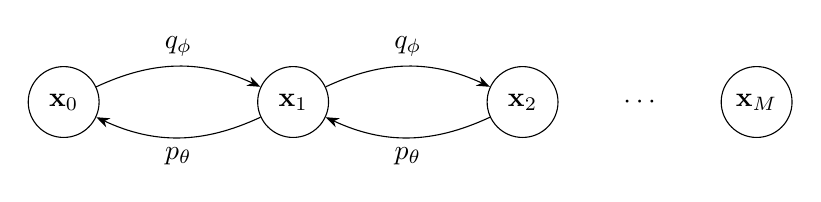
\begin{tikzpicture}[>=Stealth, node distance=2.0cm]
      \tikzset{state/.style={circle,draw,minimum size=9mm,inner sep=1pt}}

      \node[state] (x0) {$\mathbf{x}_0$};
      \node[state, right=of x0] (x1) {$\mathbf{x}_1$};
      \node[state, right=of x1] (x2) {$\mathbf{x}_2$};

      \node[right=0.7cm of x2] (xdots) {$\cdots$};
      \node[state, right=0.7cm of xdots] (xM) {$\mathbf{x}_M$};

      \draw[->, bend left=25] (x0) to node[above] {$q_\phi$} (x1);
      \draw[->, bend left=25] (x1) to node[below] {$p_\theta$} (x0);

      \draw[->, bend left=25] (x1) to node[above] {$q_\phi$} (x2);
      \draw[->, bend left=25] (x2) to node[below] {$p_\theta$} (x1);
    \end{tikzpicture}
  \end{center}

  \textbf{ELBO for MHVAEs}:
  \BA{
    \log p(\vbx_0)
    &=\log\int p_\theta(\vbx_{0:T})\d\vbx_{1:T} \\
    &=\log \Ep{q_\phi(\vbx_{1:T}\mid \vbx_0)}{\f{p_\theta(\vbx_{0:T})}{q_\phi(\vbx_{1:T}\mid \vbz)}} \\
    &\geq \Ep{q_\phi(\vbx_{1:T}\mid \vbx_0)}{\log\f{p_\theta(\vbx_{0:T})}{q_\phi(\vbx_{1:T}\mid \vbz)}}
  }

  \begin{figure}[h]
    \centering
    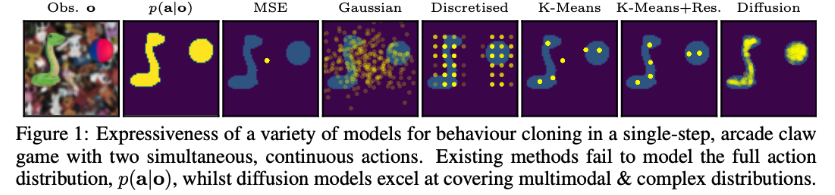
\includegraphics[width=0.90\textwidth]{figures/diffusion-comparison.png}
    \caption{Figure 1 from \textit{Imitating Human Behaviour with Diffusion Models} by Pearce \textit{et. al.}}
    \label{fig:diffusion-comparison}
  \end{figure}

  \hl{\textbf{Diffusion Models}} \cite{ho2020denoising}: A generative model that allows for greater expressivity for generating conditional distributions (Figure \ref{fig:diffusion-comparison}). Diffusion Models are MHVAE where the latent dimension is equal to the data dimension, and encoder is fixed by hyperparameters s.t. the $x_T\sim\calN(0,1)$. Specifically,
  \BA{
    q(\vbx_t\mid \vbx_{t-1})&=\calN(x_t;\sqrt{\alpha_t}\vbx_{t-1},(1-\alpha_t)I) \\
    p_\theta(\vbx_{t-1}\mid \vbx_t)&=\calN(\vbx_{t-1};\mu_\theta(x_t,t),\sigma_t^2I).
  }
  Note that $\mu_\theta$ now takes in the step $t$ as an input.
  \BI{
  \item Because the sum of Gaussian distributions is also Gaussian, we can derive tthat 
    \BE{
      q(\vbx_t\mid \vbx_0)=\calN(\sqrt{\overline{\alpha_t}}\vbx_0,(1-\overline{\alpha_t})I)
    }
    where $\overline{\alpha_t}=\prod_{i=1}^t \alpha_i$.
  \item Note that as $t\to\infty$, we have that $\overline{\alpha_t}\to 0$ so $q(\vbx_t\mid \vbx_0)\Rightarrow \calN(0,I)$.  
  }

  \textbf{ELBO for Diffusion Models}: 
  \BA{
    \log p(\vbx)
    &=\log \int p(\vbx_{0:T})\d \vbx_{1:T} \\
    &=\log \int\f{p(\vbx_{0:T})q(\vbx_{1:T}\mid \vbx_0)}{q(\vbx_{1:T}\mid \vbx_0)}\d \vbx_{1:T} \\
    &=\log \Eb_{q(\vbx_{1:T}\mid \vbx_0)}\f{p(\vbx_{0:T})}{q(\vbx_{1:T}\mid \vbx_0)} \\
    &\geq\Eb_{q(\vbx_{1:T}\mid \vbx_0)}\log\f{p(\vbx_{0:T})}{q(\vbx_{1:T}\mid \vbx_0)} \\
    &=\Eb_{q(\vbx_{1:T}\mid \vbx_0)}\log\f{p(\vbx_T)\prod_{t=1}^T p_\theta(\vbx_{t-1}\mid \vbx_t)}{\prod_{t=1}^T q(\vbx_t\mid \vbx_{t-1})} \\
    &=\Eb_{q(\vbx_{1:T}\mid \vbx_0)}\log \f{p(\vbx_T)p_\theta(\vbx_0\mid \vbx_1)\prod_{t=1}^{T-1} p_\theta(\vbx_{t}\mid \vbx_{t+1})}{q(\vbx_T\mid \vbx_{T-1})\prod_{t=1}^{T-1} q(\vbx_t\mid \vbx_{t-1})} \\
    &=\Ep{q(\vbx_{1:T}\mid \vbx_0)}{\log \f{p(\vbx_T)p_\theta(\vbx_0\mid \vbx_1)}{q(\vbx_T\mid \vbx_{T-1})}}+\Ep{q(\vbx_{1:T}\mid \vbx_0)}{\log \prod_{t=1}^{T-1}\f{p_\theta(\vbx_t\mid \vbx_{t+1})}{q(\vbx_t\mid \vbx_{t-1})}} \\
    &=\Ep{q(\vbx_{1:T}\mid \vbx_0)}{\log p_\theta(\vbx_0\mid \vbx_1)}+\Ep{q(\vbx_{1:T}\mid \vbx_0)}{\log \f{p(\vbx_T)}{q(\vbx_T\mid \vbx_{T-1})}}+\sum_{t=1}^{T-1} \Eb_{q(\vbx_{1:T}\mid \vbx_0)}\log \f{p_\theta(\vbx_t\mid \vbx_{t+1})}{q(\vbx_t\mid \vbx_{t-1})} \\
    &=\Ep{q(\vbx_{1:T}\mid \vbx_0)}{\log p_\theta(\vbx_0\mid \vbx_1)}+\Ep{q(\vbx_{T-1},\vbx_{T}\mid \vbx_0)}{\log \f{p(\vbx_T)}{q(\vbx_T\mid \vbx_{T-1})}}+\sum_{t=1}^{T-1} \Eb_{q(\vbx_{t-1},\vbx_t,\vbx_{t+1}\mid \vbx_0)}\log \f{p_\theta(\vbx_t\mid \vbx_{t+1})}{q(\vbx_t\mid \vbx_{t-1})} \\
    &=
    \underbrace{\Ep{q(\vbx_{1:T}\mid \vbx_0)}{\log p_\theta(\vbx_0\mid \vbx_1)}}_\text{reconstruction term}
    -\underbrace{\Ep{q(\vbx_{T-1}\mid \vbx_0)}{\calD_\text{KL}(q_(\vbx_T\mid \vbx_{T-1})\Vert p(\vbx_T))}}_\text{prior matching term} \\
    &\quad-\underbrace{\sum_{t=1}^{T-1} \Eb_{q(\vbx_{t-1},\vbx_{t+1}\mid \vbx_0)}\calD_\text{KL}(q(\vbx_t\mid \vbx_{t-1})\Vert p_\theta(\vbx_t\mid \vbx_{t+1}))}_\text{consistency term}
  }
  \BI{
  \item The \textbf{reconstruction term} is the same as the ELBO for VAEs given the first step latent.
  \item The \textbf{prior matching term} has no trainable parameters and ensures that the final latent distribution matches the Gaussian prior.
  \item The \textbf{consistency term} ensures that the distribution of $\vbx_t$ obtained from transitioning from noiser samples $\vbx_{t+1}$ matches the distribution over $\vbx_t$ obtained from noising cleaner samples $\vbx_{t-1}$ for all $t$. 
  }

  \textbf{ELBO for Diffusion Models Form 1}: We have that
  \BA{
    q(\vbx_{t-1}\mid \vbx_t,\vbx_0)
    &=\f{q(\vbx_t\mid \vbx_{t-1},\vbx_0)q(\vbx_{t-1}\mid \vbx_0)}{q(\vbx_t\mid \vbx_0)} \\
    &=\f{\calN(\vbx_t;\sqrt{\alpha_t} \vbx_{t-1},(1-\alpha_t)\mathbf{I}))\calN(\vbx_{t-1};\sqrt{\overline{\alpha}_{t-1}}\vbx_0,(1-\overline{\alpha}_{t-1}\mathbf{I}))}{\calN(\vbx_t;\sqrt{\overline{\alpha}_t}\vbx_0,(1-\overline{\alpha}_t)\mathbf{I})} \\
    &\propto \calN\bpa{\vbx_{t-1};\f{\sqrt{\alpha_t}(1-\overline{\alpha}_{t-1})\vbx_t+\sqrt{\overline{\alpha}_{t-1}}(1-\alpha_t)\vbx_0}{1-\overline{\alpha}_t},\f{(1-\alpha_t)(1-\overline{\alpha}_{t-1})}{1-\overline{\alpha}_t}\mathbf{I}} \\
    &=\calN(\mu_q(\vbx_t),\Sigma_q(t)), 
  }
  so the prior matching term becomes 
  \BA{
    &\sum_{t=2}^{T} \Eb_{q(\vbx_t\mid\vbx_0)}\calD_\text{KL}(q(\vbx_t\mid \vbx_{t},\vbx_0)\Vert p_\theta(\vbx_{t-1}\mid \vbx_{t})) \\
    &=\f{1}{2}\bbb{\log\f{\bab{\Sigma_y}}{\bab{\Sigma_x}}-d+\mathrm{tr}(\Sigma_y^{-1}\Sigma_x)+(\mu_y-\mu_x)^\top \Sigma_y^{-1}(\mu_y-\mu_x)} \\
    &=\f{1}{2\sigma^2_q(t)}\bbb{\bnm{\mu_\theta-\mu_q}_2^2}
  }
  where $\sigma_q^2(t)=\f{(1-\alpha_t)(1-\overline{\alpha}_{t-1})}{1-\overline{\alpha}_t}$ because the variances of both Gaussians match exactly. Here, $\mu_q(\vbx_t,\vbx_0)$ denotes the noised mean and $\mu_\theta(\vbx_t)$ denotes the denoised mean. The denoising transition mean can be rewritten as
  \BE{
    \mu_\theta(x_t,t)=\f{\sqrt{\alpha_t}(1-\overline{\alpha}_{t-1})\vbx_t+\sqrt{\overline{\alpha}_{t-1}}(1-\alpha_t)\hat{x}_\theta(\vbx_t,t)}{1-\overline{\alpha}_t},
  }
  so the overall consistency term can be written as
  \BE{
    \argmin_\theta \Eb_{t\sim U[2,T]}\Ep{q(\vbx_t\mid \vbx_0)}{\f{1}{2\sigma^2_q(t)}\f{\overline{\alpha}_{t-1}(1-\alpha_t)^2}{(1-\overline{\alpha}_t)^2}\bnm{\hat{x}(\vbx_t,t)-\vbx_0}_2^2}.
  }

  \textbf{ELBO for Diffusion Models Form 2}: Recall that
  \BA{
    q(\vbx_t\mid \vbx_0)&=\calN{\vbx_t;\sqrt{\overline{\alpha}_t}\vbx_0,(1-\overline{\alpha}_t)\mathbf{I}} \\
    \vbx_t&=\sqrt{\overline{\alpha}_t}\vbx_0+\sqrt{1-\overline{\alpha}_t}\vec{\epsilon}_0
  }
  which gives that
  \BE{
    \vbx_0=\f{\vbx_t-\sqrt{1-\overline{\alpha}_t}\vec{\epsilon}_0}{\sqrt{\overline{\alpha}_t}}.
  }
  Then,
  \BA{
    \vec{\mu}_q(\vbx_t,\vbx_0)
    &=\f{\sqrt{\alpha_t}(1-\overline{\alpha}_{t-1})\vbx_t+\sqrt{\overline{\alpha}_{t-1}}(1-\alpha_t)\vbx_0}{1-\overline{\alpha}_t} \\
    &=\f{\vbx_t}{\sqrt{\alpha_t}}-\f{1-\alpha_t}{\sqrt{1-\overline{\alpha}_t}\sqrt{\alpha_t}}\vec{\epsilon}_0.
  }
  Similarly, the denoising transition mean can be rewritten as
  \BE{
    \vec{\mu}_\theta(\vbx_t,t)=\f{\vbx_t}{\sqrt{\alpha_t}}-\f{1-\alpha_t}{\sqrt{1-\overline{\alpha}_t}\sqrt{\alpha_t}}\hat{\epsilon}(\vbx_t,t).
  }
  Thus, the consistency term reduces to
  \BE{
    \argmin_\theta \Eb_{t\sim U[2,T]}\Ep{q(\vbx_t\mid \vbx_0)}{\f{1}{2\sigma^2_q(t)}\f{(1-\alpha_t)^2}{(1-\overline{\alpha}_t)\alpha_t}\bnm{\vec{\epsilon}_0-\hat{\epsilon}_\theta(\vbx_t,t)}_2^2},
  }
  where $\epsilon_0\sim\calN(0,\mathbf{I})$ and $\hat{\epsilon}_\theta$ is a neural network parameterized by $\theta$ that predicts the noise level at step $t$. Training becomes performing gradient decent on
  \BE{
    \nabla_\theta \bnm{\vec{\epsilon}-\hat{\epsilon}_\theta(\sqrt{\overline{\alpha}_t} \vbx_0+\sqrt{1-\overline{\alpha}_t}\vec{\epsilon},t)}_2^2,
  }
  a standard least-squares objective. Then, sampling can be performed by taking $\vbx_T,\vbz_1,\dots,\vbz_T\overset{\text{iid}}{\sim}\calN(0,\mathbf{I})$ and setting
  \BE{
    \vbx_{t-1}=\f{1}{\sqrt{\alpha_t}}\bpa{\vbx_t-\f{1-\alpha_t}{\sqrt{1-\overline{\alpha}_t}}\vec{\epsilon}_\theta(\vbx_t,t)}+\sigma_t\vbz
  }

  \textbf{Conditional Diffusion Models}: Conditional diffusion models add arbitrary conditioning information $y$ at each transition step:
  \BE{
    p(\vbx_{0:T}\mid y)=p(\vbx_T)\prod_{t=1}^T p_\theta(\vbx_{t-1}\mid \vbx_t,y).
  }

\section{Model-Based Reinforcement Learning}
  
  \textbf{Online Planning}: Learning strategy where a model of the environment is rolled out to directly predict consequences of actions in order to search for the best actions to take in the current state.
  \BI{
  \item This is relevant in environments with large state-spaces where computing a good value function is difficult offline. Conditioning on the current state and estimating the value function of the relevant parts of the state space is a more efficient way to allocate resources. 
  }

  \textbf{Exhaustive Search}: An online planning branching search strategy where the current state of the agent is the root of a search tree. This is infeasible because of the large tree branching factor and large tree depth. 

  \textbf{Monte-Carlo Search}: A variant of exhaustive search that samples random trajectories. The estimated value of each state is then the average outcome from trajectories starting at that state. Formally, for a root state $s$, a deterministic transition function $T$, and a (potentially random) simulation policy $\pi$, we simulate $k$ episodes
  \BE{
    \bbr{s,a,R_1^k,S_1^k,R_2^k,S_2^k,A_2^k,\dots,S^k_T}_{k=1}^K\sim T,\pi
  }and evaluate the action value function of the root by mean return:
  \BE{
    Q(s,a)=\f{1}{K}\sum_{k=1}^K G_k
  }
  which converges to $q_\pi(s,a)$ as $K\to\infty$. Then, the action in the current state is selected via $a=\argmax_{a} Q(s,a)$. 

  \textbf{Upper Confidence Bound (UCB)}: An alternative to $\epsilon$-greedy for balancing exploration and exploitation. The action selection is weighted by
  \BE{
    w_t=\argmax_a Q_t(a)+c\sqrt{\f{\log t}{N_t(a)}}
  }
  where $t$ is the number of times the parent node has been visited, $N_t(a)$ is the number of times the action has been tried. 

  \textbf{Monte-Carlo Tree Search (MCTS)}: We maintain action values $Q$ for the root and nodes internal to a tree expanded through the course of the search. This is used to improve the simulation policy over time. Outside this tree, there are no $Q$ estimates and we fall back on a random policy. 

  Formally, MCTS consists of a \textbf{bandit phase} and a \textbf{random phase}. If a node has an unexpanded child, we expand the child (adding it to the tree) and play it out using a random policy. Otherwise, sample a child using UCB and recurse. Each node tracks the number of visits and the average return. 

  \textbf{Offline MCTS \cite{guo2014deep}}: Uses MCTS for $Q$ value estimation and action selection at training time. A reactive policy network that imitates the MCTS planner is used at test time. The authors introduces two strategies:
  \BI{
  \item \texttt{UCTtoRegression}: A regression network that regresses to $Q(s,a,w)$ for all actions and selects actions by taking the argument max.
  \item \texttt{UCTtoClassification}: A classifiaction network that, given the same context, directly predicts the best action.
  }
  The naive approach of generating $(s,a,Q(s,a))$ tuples is insufficient because the policy state distribution and the MCTS state distribution will diverge. Instead, the \textbf{interleaved method} alternates between deploying the learned $\epsilon$-greedy policy to collect trajectories, then uses MCTS as an expert to decide the best action for each state. Then, the learned policy is updated using the optimal actions. 

  \textbf{MCTS with Policy/Value Networks}: MCTS can be optimized by using a value network to evaluate board positions to prune the tree depth, and a policy networks to select moves and prune the tree breadth.
  \BI{
  \item Similar to Actor-Critic, these can be trained jointly with a state embedding with separate heads to predict the action and value function. 
  }

  \textbf{AlphaGo \cite{silver2016mastering}}: First, train cheap policy $p_\pi$ and expersive policy $p_\sigma$ using imitation learning on human expert games. Then, train a new policy $p_\rho$ with RL and self-play initialized from the $p_\sigma$ policy. Train a value network $V_\theta$ that predicts the winner of games played by $p_\rho$ against itself. At test time, MCTS is used to select the best move. 

  The action selection policy of the MCTS is given by
  \BE{
    a_t=\argmax_a Q(s_t,a)+c\sqrt{N(s_t)}\f{\pi_\theta(a_t\mid s_t)}{1+N(s_t,a_t)}
  }
  where $\pi_\theta(a\mid s)$ is the prior expert probabilities provided by $p_\sigma$, $Q(s_r,a)$ is the average reward collected so far from MC simulations, and $N(s,a)$ is the number of times action $a$ has been taken in state $s$. A leaf node $L$ is evaluated as
  \BE{
    V(s_L)=(1-\lambda)V_\theta(s_L)+\lambda z_L
  }
  where $z_L$ is the roward from the fast rollout $p_\pi$ (done in parallel) and $\lambda$ isa mixing parameter. Once the MCTS completes, the algorithm chooses the most visited move from the root position. 

  \textbf{AlphaGoZero \cite{silver2017mastering}}: AlphaGo with ``zero'' human examples to seed the policy, due to having a better training loop to discover stronger actions in training using offline MCTS. The UCB during training is the same as the base AlphaGo, except the policy $\pi_\theta(a_t\mid s_t)$ is changing during the policy. Once MCTS completes, the algorithm  trains the policy $\pi_\theta$ against the visit distribution $\hat{\pi}$:
  \BA{
    \hat{\pi}(a)&=\f{n(a)}{\sum_{a'} n(a')}.
  }
  Then, the next action for the self-play loop is sampled from $\hat{\pi}$ to encourage exploration. The value function is simply regressed to the outcome of the game. 
  \BI{
    \item
      Motivation: From Hamrick \textit{et. al.} \cite{hamrick2020role}, planning is more important at training time because it leads to more intelligent exploration.
    \item
      Value function approximations are used for leaf nodes (no full rollouts). Value functions are only updated when the game terminates. This techinque is called the \textbf{terminal value function}.
    \item
      Note that the neural network has a single backbone that accepts a state input, and two heads that predict the action distribution and the value function.
    \item
      Similarly to AlphaGo, MCTS is still used a test-time. 
  }

\section{Model-Free Reinforcement Learning}
  \textbf{Model-Free Reinforcement Learning}: Policy interacts with a learned model of the environement (dynamics $p(s_{t+1}\mid s_t,a_t)$ and $r(s_t,a_t)$ are simulated/learned). This can be done using neural networks, Gaussian processes, etc. 
  \BI{
  \item Models are useful for lookahead, such as MCTS, or used for synthetic experience generation that augments real experience to boost a model-free algorithm such as PPO.
  \item Goal is to have high rewards with little interactions with the actual environment. 
  }

  \textbf{MBRL with Learned Models}: We first run the policy and update experience tuples dataset $\calD_\text{env}$. Then, the dynamics model is regressed to $\calD_\text{env}$:
  \BE{
    \min_f \Eb_{s_t,a_t,s_{t+1}\sim \calD_\text{env}} \bnm{s_{t+1}-f(s_t,a_t)}.
  }
  Then the policy is optimized using rollouts from the learned function $f$.
  \BI{
  \item State distribution mismatch is a big problem here because any mismatch between $f$ and the ground truth will be exploited by the policy. 
  \item In practice, the difference between the current state and next state is modelled: $s'=s+f_\phi(s,a)$
  \item The reward in this case is defined as the distance to some final state $s^*$.
  }

  \textbf{Model-predictive Control (MPC)}: An instance of MBRL with Learned Models where an action is executed sequentially, the following state is observed, and the model replans for future steps. This mitigates the problem of error accumulation through unrolling. 

  \textbf{MBRL in Low-Dimensional States}: The state is observed and given in low-dimensional space (e.g., object locations and robot configurations).  

  \textbf{MBRL from High-Dimensional Sensory Input}: The state is observed and given in terms of high-dimensional sensory input such as video. The two approaches to addressing this is recurrence on image space (e.g., deterministc video prediction) or recurrence in latent space. 

\subsection{MBRL in State-Space}

  \textbf{Probabilistic Ensembles with Trajectory Sampling (PETS) \cite{chua2018deep}}: Model representations of the environment are augmented with uncertainty predictions. Specifically, there are two types: \textbf{epistemic uncertainty} is due to the lack of data (e.g., for a deterministic system), and \textbf{aleatoric uncertainty} is due to the inherent stochasticity of the system The model outputs a Gaussian distribution over next states given the current state and action by predicting the mean and covariance matrix:
  \BE{
    \calL_\phi = -\f{1}{N} \sum_{i=1}^N \log p_\phi(s_i'\mid s_i,a_i).
  }
  An ensemble of networks ($3$ networks) is used to make this prediction in parallel; the variance of the results across the ensemble estimates the epistemic uncertainty. The reward of an action sequence is done by averaging across \textbf{particles}, where each particle is a separate network.
  \BI{
    \item Aleatoric uncertainty implies that standard regressive predictions will not perform well and motivates the use of architectures capable of handling multi-modality such as diffusion networks.
    \item Use $\ln$-$\exp$ trick to predict positive values for variances. 
  }

  The final algorithm is: Use the cross-entropy method (an evolutionary search algorithm) to optimize over action sequences $a^*_{t,\dots,T}$ by unrolling the model ensemble and reward averaging, executing the first action $a^*_t$ and updating the environment dataset $\calD_\text{env}$ with tuple $(s_t,a_t^*,s_{t+1})$.
  \BI{
  \item Suppose there are $B$ models in the ensemble. In CEM, we first sample an action sequence $\vva_{t\dots T}$ from the learned action sequence distribution. For each model $b\in\bbr{1,\dots,B}$, set $s_t^{(b)}=s_t$ and compute for each following step,
    \BA{
      s_{k+1}^{(b)}&\sim p_k(s_k^{(b)},a_k) \\
      r_k^{(b)} &= r(s_k^{(b)}, a_k) \\
      R^{(b)}(\vva)&=\sum_{k=t}^T r(s_k^{(b)},a_k)
    }
    Then, the return for $\vva$ is said to be the average across all $R^{(b)}(\vva)$. Note that the states are not averaged across ensembles.
  }

\subsection{MBRL in Sensory-input Space}

  \textbf{Approaches to MBRL in Sensory-input Space}: There are two main approaches to MBRL in sensory-input space:
  \BI{
  \item
    \textbf{Unrolling in the observation space}: The environment model is given observations $o_{t-k},\dots,o_t, a_t$ and asked to predict $o_{t+1}$.
  \item
    \textbf{Unrolling in the latent space}: The environment model is given a latent state $s_t$ representing observations $o_{t-k},\dots,o_t$ as well as $a_t$ and asked to predict $s_{t+1}$. 
  }

  \textbf{Action-Conditional Video Predicting using Deep Networks in Atari Games \cite{oh2015action}}: Trains a neural network that given an image sequence and an actions, predicts the pixels of the next frame using a standard $L_2$ objective. Using a naive approach, we face the problem of \textbf{error accumulation} where test-time rollouts have a distribution shift (similar to imitation learning). This can be solved by:
  \BN{
  \item Progressively unrolling the horizon $k$ at training time so that the model learns to handle its mistakes:
    \BE{
      \calL(\theta)=\f{1}{N} \sum_{i=1}^N \bnm{f(a^{(i)}_{t+1}, f(a^{(i)}_t,o^{(i)}_t;\theta);\theta)-o^{(i)}_{t+2}}+\bnm{f(a^{(i)}_t,o^{(i)}_t;\theta)-o^{(i)}_{t+1}}.
    }
    This fails for non-regressive, multi-modal models and highly stochastic environments because the model rollout and the ground truth and deviate significantly.
  \item Add noise to each observation to simulate predictions of the networks. 
  }

  \textbf{Model-Based Reinforcement Learning for Atari \cite{kaiser2019model}}: Similar architecture to before but also make predictions on rewards: First initialize $\pi_\theta$ and $\calD_\text{env}$. In each iteration, run the policy and update $\calD_\text{env}$. Then, train the dynamics model by regressing $f(\{o_{t-4},\dots,o_t\},a_t,z;\theta)$ to $(o_{t+1}, r_{t+1})$. Then, sample $o_{t-4},\dots,o_t\sim \calD_\text{env}$ and collect simulated experience $\calD_\text{model}$ for $50$ time steps using $\pi_\theta$ to select actions. Finally, update $\pi_\theta$ using PPO on trajectories $\calD_\text{model}\cup \calD_\text{env}$. 
  \BI{
  \item The paper uses a multi-model VQ-VAE for $f(\cdot;\theta)$. This inherently operates similar to an ensemble by encorporating epistemic uncertainty, which mitigates the need to use an actual ensemble (as used in PETS). 
  \item Compared to a base model-free PPO model, the model-based method required much less (actual) environment interactions to read human-level performance.
  \item Disadvantages: video prediction loss does not reflect task performance (predicts task-irrelevant objects), and is extremely slow. 
  }

  \textbf{Temporal Difference for Model Predictive Control (TD-MPC) \cite{hansen2022temporal}}: Train an encoder $E_\phi$ and a decoder $D_\psi$ with an autoencoder loss
  \BE{
    \min_{\phi,\psi} \bnm{D_\psi(E_\phi(o_t))-o_t}.
  }
  The encoder also encoporates task-relevant losses such as action prediction, reward prediction, and $Q$-value prediction. Then, the dynamics prediction is performed entirely on the latent space:
  \BE{
    \min_\theta \bnm{f_\theta(E_\phi(o_{t-K}),\dots,E_\phi(o_t))-E_\phi(o_{t+1})}.
  }

  \textbf{Tasked-Oriented Latent Dynamics (TOLD)}: TOLD minimizes the objective
  \BE{
    \calJ(\theta;\Gamma)=\sum_{i=t}^{t+H} \omega^{i-t} \calL(\theta;\Gamma_i)
  }
  where
  \BA{
    \calL(\theta;\Gamma_i)
    &=\lambda_1\underbrace{\bnm{R_\theta(\vbz_i,\vva_i)-r_i}_2^2}_\text{reward} \\
    &\;+\lambda_2\underbrace{\bnm{Q_\theta(\vbz_i,\vva_i)-(r_i+\gamma Q_{\theta^-}(\vbz_{i+1},\pi_\theta(\vbz_{i+1})))}_2^2}_\text{value} \\
    &\;+\lambda_3\underbrace{\bnm{d_\theta(\vbz_i,\vva_i)-h_{\theta^-}(\vvs_{i+1}))}_2^2}_\text{latent state consistency}.
  }
  Here, $\theta^-$ represent the parameters of a target network that is a moving average of $\theta$. Then, the policy minimizes
  \BE{
    \calJ_\pi(\theta;\Gamma)=-\sum_{i=t}^{t+H} \omega^{i-t}Q_\theta(\vbz_i,\pi_\theta(\mathrm{sg}(\vbz_i))),
  }
  where the $\mathrm{sg}$ operator represents stop-gradient, preventing the gradient from updating the latent state encoder.

  \textbf{Planning in Latent-Space}: We can estimate the return of a trajectory via
  \BE{
    \Eb_{\Gamma}\;\underbrace{\gamma^HQ_\theta(\vbz_H,\vva_H)}_\text{value}+\underbrace{\sum_{t=0}^{H-1} \gamma^t R_\theta(\vbz_t,\vva_t)}_\text{rewards}.
  }
  This is used to maximize an evolutionary search method such as CEM (similar to PETS, but with a different dynamics model and a terminal value function).  

  \textbf{Planning with a Learned Model (MuZero) \cite{schrittwieser2020mastering}}: For a given game state encodes each observation with a learned encoder $h_\theta(o_1,\dots,o_t)=s^{(0)}$. Then, a prediction network predicts a distribution over actions and a state value $f_\theta(s^{(k)})=(\vvp^{(k)},\nu^{(k)})$. Finally, the learned dynamics function gives $g_\theta(s^{(k-1)},a^{(k)})=(r^{(k)},s^{(k)})$. 

  Doing this process in a tree search similar to AlphaZero gives an improved policy (action distribution by normalizing visitation counts) and an improved value function (average $Q$s over actions). Note that the tree search is executed with the actual environment, not the learned simulator.
  \BI{
    \item
      The learned model update is by regressing the state embedding to match the policy, reward, and $n$-step value bootstrap:
      \BE{
        v_t\approx u_{t+1} + \gamma u_{t+2} + \cdots + \gamma^{n-1} u_{t+n} + \gamma^n \nu_{t+n},
      }
      where the last term is the improved state value estimate the MCTS. Note that a decoding is not required or helpful. A consistency loss can also be added. 
  }

  \textbf{MuZero Reanalyze \cite{schrittwieser2021online}}: We can reuse old trajectories by again training policy and reward to its corresponding values $p_t\to \pi_t^{T'}$, $r_t\to u_t^T$. Instead of $n$-step bootstrapping, because the trajectory is now modified, we just directly update with MCTS $v_t\to \nu_t^{T''}$, where $T$ represents the trajectory in the ground-truth environment, $T'$ is the original sampled trajectory in the latent state, and $T''$ is the reused trajectory generated by post-training with MCTS.  
  \BI{
    \item
      This can increase replay by $10\times$, using only $10\%$ new trajectories with $90\%$ reanalyzed old trajectories.
    \item 
      Only offers a significant advantage over MuZero in strategy games where planning in relevant (e.g. Chess, Go, but not Pacman).
  }

\subsection{MBRL with Guided Diffusion}

  \textbf{Score function}: The score function of a distribution is given by $\nabla_{\vbx} \log p(\vbx)$. This defines a vector field over the entire data space, and performing gradient ascent on this field leads to data modes.

  \textbf{Tweedie's Formula}: For a Gaussian variable $\vbz\sim\calN(\mu_{\vbz},\Sigma_{\vbz})$, we have that
  \BE{
    \Ec{\vec{\mu}_{\vbz}}{\vbz}=\vbz+\Sigma_{\vbz}+\nabla_{\vbz}\log p(\vbz).
  }

  \textbf{Predicting the Score with Diffusion Models}: Tweedie's formula enables the prediction of the true posterior mean $\vbx_t$ given its samples. Given that
    \BE{
      q(\vbx_t\mid \vbx_0)=\calN(\vbx_t;\sqrt{\overline{\alpha_t}\vbx_0,(1-\overline{\alpha}_t\vbI)}),
    }
    we have that 
    \BE{
      \Ec{\mathbf{\mu}_{\vbx_t}\mid \vbx_t}=\vbx_t+(1-\overline{\alpha}_t)\nabla_{\vbx_t}\log p(\vbx_t).
    }
    Since $\mathbf{\mu}_{\vbx_t}=\sqrt{\overline{\alpha}_t}\vbx_0$, we have that
    \BE{
      \vbx_0=\f{\vbx_t+(1-\overline{\alpha}_t)\nabla \log p(\vbx_t)}{\sqrt{\overline{\alpha}_t}}.
    }
    We also have that for some $\mathbf{\epsilon}_0\sim\calN(0,\vbI)$, that
    \BE{
      \vbx_t=\sqrt{\overline{\alpha}_t}\vbx_0+\sqrt{1-\overline{\alpha}_t}\mathbf{\epsilon}_0.
    }
    Solving for $\vbx_0$ and equating the two expressions gives a score function of
    \BE{
      \nabla\log p(\vbx_t)=-\f{1}{\sqrt{1-\overline{\alpha}_t}}\mathbf{\epsilon}_0.
    }
    Since this is the direction in the data space to add noise to the image, we move in the opposite direction to increase the log probability. Note that at generation time, we approximate $\mathbf{\epsilon}_0$ with $\epsilon_\theta(\vbx_t,t)$.

  \textbf{Conditional Diffusion Generation}: Suppose we then try to condition the generation process on some data $y$. We have that
  \BA{
    \nabla\log p(\vbx_t\mid y)
    &=\nabla\log \f{p(\vbx_t)p(y\mid \vbx_t)}{p(y)} \\
    &=\nabla\log p(\vbx_t)+\nabla\log p(y\mid \vbx_t)-\nabla\log p(y).
  }
  Taking the argmax eliminates the last term because it does not depend on the data.
  \BI{
    \item 
      The distribution $p(y\mid \vbx_t)$ is a simple classifier. Note that this needs to be trained on both clean and noised images.
    \item
      The two terms can be weighted as follows:
      \BE{
        \nabla_\vbx \log p_\gamma(\vbx\mid y)=\nabla_\vbx\log p(\vbx)+\gamma\nabla_\vbx\log p(y\mid\vbx).
      }
  }

  \textbf{Model-based RL with Diffusion Models}: We represent trajectories as sing-channel images and train a diffusion model to iteratively denoise the entire trajectory. Sampling is done by iteratively refining randomly-initialized trajectories.
  \BI{
    \item
      Such a diffuser is implemented with one-dimensional convolutions for temporal equivariance and horizon independence.
    \item
      Note that prediction is \textbf{non-autoregressive} since the entire trajectory is predicted simultaneously.
  }
  The trajectory is then guided with learned value/cost functions:
  \BE{
    \tilde{p}_\theta(\boldsymbol{\tau})\propto p_\theta(\boldsymbol{\tau}) h(\boldsymbol{\tau}),
  }
  corresponding to the behavior model, the diffusion model, and the guidance function, respectively.

  \textbf{Goal Planning through Inpainting}: Suppose the guidance function specifies only the initial and goal states. Then, a straightforward method is to substitute $s_0^{(t)}$ and $s_n^{(t)}$ with the initial and goal states, respectively, at each denoising time step.

  \textbf{Model-based Control with Generative Trajectory Models}: First, we train a diffusion model by minimizing the MSE between predicted and true noised trajectory:
  \BE{
    \argmin_\theta \calL(\theta)=\bab{\epsilon_\theta(\vbx_t,t)-\epsilon_t}^2.
  }
  Then, generation is preformed by sampling $\vbx_T\sim\calN(0,\vbI)$ and performing:
  \BA{
    \vbx_{0\mid t}&=\f{1}{\sqrt{\overline{\alpha}_t}}\bpa{\vbx_t-\sqrt{1-\overline{\alpha}_t}\epsilon_\theta(\vbx_t,t)} \\
    \vbx_{0\mid t}^\text{guided}&=\vbx_{0\mid t}+c_t\nabla_{\vbx_{0\mid t}}r(\vbx_{0\mid t}) \\
    \vbx_{t-1}&=\sqrt{\overline{\alpha}_{t-1}}\vbx_{0\mid t}^\text{guided}+\sqrt{1-\overline{\alpha}_{t-1}-\sigma_t^2}\epsilon_\theta(\vbx_t,t)+\sigma_t\epsilon
  }
  Note that the roward function $r$ here needs to be both diffentiable and trained on both unnoised/noised trajectories.

  \textbf{Diffusion-ES}: Standard ES requires a mutation operator, which is typically of the form $x'=x+\sigma\boldsymbol{\epsilon}$, which likely deviates from the manifold of valid trajectories. Diffusion-ES instead partially noises the trajectories via
  \BE{
    \overline{x}=\sqrt{\overline{\alpha}_{n_k}}\vbx+\sqrt{1-\overline{\alpha}_{n_k}}\boldsymbol{\epsilon}
  }
  for $\boldsymbol{\epsilon}\sim\calN(0,\vbI)$ and then denoises via $x'\sim p_\theta(x\mid\overline{x})$.


\section{Offline Reinforcement Learning}

  \textbf{Offline/Batch Reinforcement Learning}: Methods that learn from a fixed experience buffer $\calD=\bbr{(s_i,a_i,s_i',r_i)}_{i=1}^k$ of state-action-reward trajectories sampled from some unknown policy $\pi_\beta$. Note that the trajectories in the buffer may have high rewards or low rewards. The goal is to compute a policy $\pi_\theta$ s.t.
  \BE{
    \max_\theta \Eb_{\tau\sim\pi_\theta}\sum_{t} r(s_t,a_t)
  }
  \BI{
  \item Offline RL methods should be able to beat a behavior cloning baseline because it has access to the rewards associated with each state-action pair. This allows it to \textbf{stitch} optimal behaviors.
  \item Offline RL is useful for incorporating existing, static datasets from non-expert policies to problems where the environment interactions are unsafe or expensive. 
  }

  \textbf{Offline RL with Actor-Critic}: One approach is to apply a standard off-policy RL algorithm like actor-critic (e.g., DDPG) to an offline dataset. This corresponds to critic updates
  \BE{
    \min_\phi \Eb_{(s,a,a')\sim\calD} \bpa{Q_\phi^\pi(s,a)-\bpa{r(s,a)+\gamma\Eb_{a'\sim \pi_\theta(\cdot\mid s')} Q_\phi^\pi(s',a')}}^2
  }
  and actor updates
  \BE{
    \max_\theta \Eb_{s\sim\calD, a\sim\pi_\theta(\cdot\mid s)} Q_\phi^\pi(s,a)
    \nabla_\theta J(\theta)=\frac{1}{N}\sum_i \nabla_\theta\log \pi_\theta(a_i^\pi\mid s_i)Q_\phi^{\pi_\theta}(s_i,a_i^\pi)
  }
  where $a_i^\pi\sim \pi_\theta(\cdot\mid s_i)$.
  \BI{
  \item Off-policy deep reinforcement learning fails when truly off-policy, even when the algorithm and base dataset are the same. This is due to \textbf{distribution shift} problem: $a'$ is sampled from the policy and out of distribution from the dataset. This leads to overestimation on OOD actions. 
  \item
    Specifically, suppose we train a reward modelr $\hat{r}_\theta(x,a)$ that approximates $r(x,a)$ in expectation under $p_\text{data}(a,x)$, but is incorrect on unseen actions. The policy then exeploits errors in this reward function.
  }

  \textbf{Filtered Behavior Cloning}: A simple baseline is to filter the dataset by taking only top trajectories by reward $\tilde{\calD}=\{\tau\mid r(\tau)>\eta\}$ and train only on those state-action pairs. 

  \textbf{Combining Behavior Cloning with TD3 \cite{fujimoto2021minimalist}}: We add a behavior cloning term to the TD3 loss to keep predicted actions close to the given actions:
  \BE{
    J(\theta)=\Ep{(s,a)\sim\calD}{-\lambda Q_\phi^{\pi_\theta}(s,\pi_\theta(s))+\bnm{\pi_\theta(s)-a}^2}
  }
  with parameters $\lambda=\alpha/\Ep{\calD}{\bab{Q(s,a)}}$ and $\alpha=2.5$. 

  \textbf{Batch-Constrained Q Learning (BCQ) \cite{fujimoto2019off}}: Constrain actions to only actions in the dataset, and only consider actions that are likely under the data distribution. This can be done with a generative model such as a conditional VAE or a diffusion model $G_\omega(a\mid s)$. Then, sample an action $a_i'\sim G_\omega(s)$ and take the action $a_i=a_i'+\xi_\phi(s,a)$ where $\xi_\phi$ adds a small perturbation near the dataset. The action taken is given by
  \BE{
    a^*=\argmax_i a_i.
  }
  The Bellman backup is similar to that of the TD3:
  \BA{
    y&=r+\gamma\max_{a_i}\bbb{\lambda \min_{j\in\bbr{1,2}} Q_{\overline{\theta}_j}(s', a_i)} \\
    \theta_j&:=\argmin_{\theta_j} \sum\bpa{Q_{\theta_j}(s,a)-y}^2 \\
    \phi&:=\argmax_\phi \sum Q_{\theta_1} (s,a+\xi_\phi(s,a))
  }
  where $a\sim G_\omega(s)$. Then, the target networks are soft-updated.

  \textbf{Conservative Q Learning \cite{kumar2020conservative}}: In conservative models, the estimated reward model $\hat{r}_\theta(x,a)$ is ``conservative'' in the sense that $\hat{r}_\theta(x,\overline{a})\leq r(x,\overline{a})$ on unseen actions. This loss is given by
  \BA{
    \min_\phi \max_\mu &\Eb_{(s,a,s')\sim\calD}\bpa{Q_\phi^\pi(s,a)-\bpa{r(s,a)+\gamma\Eb_{a'\sim\pi_\theta(\cdot\mid s')} Q_\phi^\pi(s',a')}}^2\\
                       &\quad +\alpha \Eb_{s\sim\calD,a\sim\mu(\cdot\mid s)} Q_\phi^\pi(s,a)-\alpha\Eb_{(s,a)\sim\calD} Q_\phi^\pi(s,a)+\Eb_{s\sim\calD}\calH(\mu(\cdot\mid s)),
  }
  where $\mu$ is an auxiliary action distribution to probe where the critic is assigning large values. The terms of the loss correspond to the standard TD learning critic update, increased loss for large $Q$-values, decreased loss for $Q$-values for in-dataset actions, and an regularization term to prevent $\mu$ from collapsing into a single argmax action.

  \BI{
    \item
      Consider finding
      \BE{
        \max_\mu \Eb_{a\sim\mu(\cdot\mid s)} Q(s,a)+\calH(\mu(\cdot\mid s))
      }
      for a fixed state $s$. The \textbf{partition function} is defined as 
      \BE{
        Z(s)=\sum_{\overline{a}}\exp Q(s,\overline{a})
      }
      Then, the Boltzmann/softmax form of the optimal distribution is expressed as
      \BE{
        \mu^*(a\mid s)=\f{\exp Q(s,a)}{Z(s)}.
      }
      taking the log and rearranging yields
      \BA{
        Q(s,a)&=\log\mu(a\mid s)+Z(s) \\
        \Eb_{a\sim\mu(\cdot\mid s)} Q(s,a)&=\Eb_{a\sim\mu(\cdot\mid s)}\log\mu(a\mid s)+\log Z(s).
      }
      Since the entropy term is exactly $\Eb_{a\sim\mu(\cdot\mid s)}\log\mu(a\mid s)$, the optimal distribution is simply
      \BE{
        Z(s)=\log\sum_a \exp Q(s, a)
      }
  }
  The new expression becomes 
  \BA{
    \min_\phi &\Eb_{(s,a,s')\sim\calD}\bpa{Q_\phi^\pi(s,a)-\bpa{r(s,a)+\gamma\Eb_{a'\sim\pi_\theta(\cdot\mid s')} Q_\phi^\pi(s',a')}}^2\\
              &\quad -\alpha\Eb_{(s,a)\sim\calD} Q_\phi^\pi(s,a)+\alpha\log\sum_{\overline{a}}\exp Q_\phi^\pi(s,\overline{a}).
  }
  The corresponding actor updates are simply given by
  \BE{
    \max_\theta \Eb_{s\sim\calD,a\sim\pi_\theta(\cdot\mid s)} Q^\pi(s,a)
  }

  \textbf{Advantage-Weighted Behavior Cloning}: A simple extension of behavior cloning to offline RL is to weight the contribution of each state-action-reward pair by their corresponding advantage:
  \BE{
    \argmax_\theta \Ep{(s,a)\sim\calD}{\log\pi_\theta(a\mid s)\exp A(s,a)}.
  }
  This requires computing advantages $A(s,a)=Q(s,a)-V(s)$ without querying OOD actions.

  \textbf{Advantage-Weighted Regression (AWR) \cite{peng2019advantage}}: Suppose the buffer is generated with some policy $\pi_\beta$. We can estimate the state-value function with Monte Carlo:
  \BA{
    V^{\pi_\beta}(s)&:=\min_\phi \Eb_{s_t\sim\calD} \bnm{V^{\pi_\beta}_\phi(s_t)-\sum_{t'=t}^T r(s_{t'},a_{t'})}^2 \\
    A^{\pi_\beta}(s_t,a_t)&:=\sum_{t'=t}^T r(s_{t'},a_{t'})-V^{\pi_\beta}_\phi(s_t)
  }
  Then, we extract the policy
  \BE{
    \hat{\theta}:=
    \argmax_\theta \Ep{(s,a)\sim\calD}{\log\pi_\theta(a\mid s)\exp\bpa{\f{1}{\beta}A^{\pi_\beta}(s,a)}}.
  }
  Here, $\beta$ is a parameter that controls the shapness of reweighting.
  \BI{
    \item
      This can be adapted to be an online off-policy algorithm by alternating between updating $\pi_\theta$ and augmenting the dataset via $\calD:=\calD\cup\bbr{\tau_i}$ sampled from $\pi_\theta$.

    \item
      Standard MC or TD learning for the $Q$ or $V$ functions reflect a mixture of policies of variable competence, when we want to extract the policy with the best performance.
  }

  \textbf{Boltzmann Reweighting of Policy}: We show that the AWR algorithm is exactly the KL-regularized policy improvement. Let $\pi$ and $\mu$ be two policies. From the performance difference lemma,
  \BE{
    J(\pi)-J(\mu)=\Eb_{\tau\sim p_\pi}\sum_{t=0}^\infty \gamma^t A^\mu(s_t,a_t)=\Eb_{s\sim d^\pi,a\sim\pi(\cdot\mid s)} A^\mu(s,a)\approx \Eb_{s\sim d^\mu,a\sim\pi(\cdot\mid s)} A^\mu(s,a),
  }
  where we assume that $\Eb_{s\sim d^\mu}\bbb{D_\text{KL}(\pi\Vert\mu)} \leq \epsilon$ for the approximation to be valid. The Lagrangian is given by
  \BA{
    \calL(\pi,\beta)
    &=\int_s d_\mu(s)\int_a \pi(a\mid s)A^\mu(s,a)\d a\d s
      -\beta\bpa{\int_s d_\mu(s) \calD_\text{KL}\bpa{\pi(\cdot\mid s)\Vert\mu(\cdot\mid s)}\d s - \epsilon} \\
    &=\int_s d_\mu(s)\int_a \pi(a\mid s)A^\mu(s,a)\d a\d s
      -\beta\bpa{\int_s d_\mu(s)\int_a \pi(a\mid s)\log\f{\pi(a\mid s)}{\mu(a\mid s)}\d a\d s - \epsilon}
  }
  Taking the functional derivative, we get that
  \BE{
    \f{\delta\calL}{\delta\pi(a\mid s)}
    = d_\mu(s)A^\mu(s,a) - \beta\, d_\mu(s)\bpa{\log\f{\pi(a\mid s)}{\mu(a\mid s)}+1}
  }
  Setting for zero and solving for $\pi$, we get
  \BE{
    d_\mu(s)A^\mu(s,a) - \beta\, d_\mu(s)\bpa{\log\f{\pi(a\mid s)}{\mu(a\mid s)}+1} = 0
  }
  \BE{
    \f{\pi(a\mid s)}{\mu(a\mid s)} = \exp\bpa{\f{1}{\beta}A^\mu(s,a)-1} = e^{-1}\cdot\exp\bpa{\f{1}{\beta}A^\mu(s,a)}
  }
  Absorb constants into normalization:
  \BE{
    \pi^*(a\mid s) \propto \mu(a\mid s)\exp\bpa{\f{1}{\beta}A^\mu(s,a)}
  }
  Then, project $\pi^*$ onto the manifold of parameterized policies:
  \BA{
    &\argmin_\pi\; \Eb_{s\sim\calD}\bbb{D_\text{KL}\bpa{\pi^*(\cdot\mid s)\Vert\pi(\cdot\mid s)}} \\
    &= \argmax_\pi\; \Eb_{s\sim d_\mu(s),\,a\sim\mu(\cdot\mid s)}\bbb{\log\pi(a\mid s)\exp\bpa{\f{1}{\beta}A^\mu}}.
  }

  \textbf{Expectile Regression}: The $\tau$-expectile is the mean with asymmetric weighting
  \BE{
    \argmin_{m_\tau} \Eb_{x\sim X} L_2^\tau(x-m_\tau)
  }
  where $L_2^\tau(u)$ is $\tau u^2$ for $u\geq 0$ and $(1-\tau)u^2$ for $u<0$. The mean is equivalent to the $0.5$-expectile.

  \textbf{Implicit Q Learning (IQL) \cite{kostrikov2021offline}}: We modify TD learning to use $L_2^\tau$:
  \BA{
    V_\psi(s)&:=\argmin_{V} \Eb_{(s,a)\sim\calD} L_2^\lambda(V(s)-Q_\phi^\calD(s,a)) \\
    Q_\phi^\calD(s,a)&:=\argmin_Q \Eb_{(s,a,s')\sim\calD} \bpa{Q(s,a)-\bpa{r(s,a)+\gamma V_\psi(s')}}^2.
  }
  The policy is extracted via AWR:
  \BE{
    \argmax_\pi \Ep{(s,a)\sim\calD}{\log\pi(a\mid s)\exp\bpa{\f{1}{\beta}\bpa{Q_\phi^\calD(s,a)-V_\psi(s)}}}.
  }

\section{Exploration}

  \textbf{$\boldsymbol{\epsilon}$-greedy Disadvantages}: The probability of identifying a favorable trajectory decreases as the number of actions and the time-horizon until the reward increases.

  \textbf{Motivation for Exploration}: Motivation can be \textbf{extrinsic}, or driven by some external reward, or \textbf{intrinsic}, being moved to do something because it is inherently enjoyable (e.g., curiosity, exploration, novelty, etc.). The latter is important because it is task independent and free of human supervision.
  \BI{
    \item
      Methods for inducing curiosity-driven exploration include: using ensembles of $Q$ functions to model uncertainty, \textbf{state counting} to approximate distributions of sampled states, measuring \textbf{model prediction error}, and measuring \textbf{reachability} from already explored states.
  }

  \textbf{Multi-armed Bandit Problem}: At each time step $t$, an agent chooses arm $k\in[K]$ and plays it, yielding reward $r_{k,t}\sim \calP_k$ where $\E{\calP_k}=\mu_k$. The distributions $\calP_k$ and means $\mu_k$ are unknown to the agent. The objective is to maximize the cumulative rewards, over a finite or infinite horizon.

  \textbf{Action-Value}: The action-value for an action $a$ is its mean reward
  \BE{
    q_*(a)=\Ec{r_t}{a_t=a}.
  }
  \BI{
    \item
      Suppose the agent forms estimates $\fa a\in\calA, Q_t(a)\approx q_*(a)$. Define the \textbf{greedy action} at time $t$ as
      \BE{
        a_t^*=\argmax_a Q_t(a).
      }
      Then, if $a_t=a_t^*$, the agent is \textbf{exploiting}; otherwise, the agent is \textbf{exploring}.
  }

  \textbf{Regret}: Let $\mu^*=\max_{a\in\mathcal{A}} \mu_a$ be the maximum expected mean reward. The cummulative regret up to time $t$ is defined as
  \BE{
    I_t=\sum_{i=1}^t \Delta_{a_i}=\sum_{i=1}^t (\mu^*-\mu_{a_t}).
  }
  Equivalently, we have that
  \BE{
    \E{I_t}=\sum_{a\in\calA} \Delta_a\E{N_a(t)}.
  }

  \textbf{Action-Value Estimates}: We focus on one action for simplicity. Suppose the rewards for the first $n-1$ timesteps are $r_1,\dots,r_{n-1}$. Then, the estimate is simply the mean:
  \BE{
    Q_n=\f{1}{n-1}(r_1+\cdots+r_{n-1}).
  }
  The online update rule is given by
  \BE{
    Q_{n+1}:= Q_n+\f{1}{n}(r_n-Q_n).
  }

  \textbf{Fixed Exploration Action Selection}: We allocate a fixed time period to explore, trying bandits uniformly at random. Then, mean rewards are formed for all actions:
  \BE{
    Q_t(a)=\f{1}{N_t(a)}\sum_{i=1}^{t-1}r_i \mathbf{1}(a_i=a)
  }
  (assuming that each bandit is a Bernoulli r.v.). Then, the action selected at each time step is the maximum among all estimated mean rewards. In an infinite horizon setting, the fixed exploration strategy will always exploit.

  \textbf{$\boldsymbol{\epsilon}$-Greedy Action Selection}: In $\epsilon$-greedy, the agent explores with probability $\epsilon$ and explores otherwise. This is the simplest way to balance exploration and exploitation. Constant $\epsilon$ produces linear total regret:
  \BE{
    I_t\geq \f{\epsilon}{K}\sum_{a\in\calA}\Delta_a,
  }
  implying that $I_t/t$ approaches a constant as $t\to\infty$.

  \textbf{Bayesian Bandits}: Bayesian bandits compute the posterior distribution of rewards
  \BE{
    p\bbb{\calR\mid a_1,r_1,\dots,a_{t-1},r_{t-1}}.
  }
  This is computed by specifying a prior $p(\calR)$ and applying Bayes' rule.

  \textbf{Thompson Sampling}: At each time step, sample from the mean reward distributions:
  \BE{
    \fa k\in[K], \overline{\theta}_k\sim\hat{p}(\theta_k).
  }
  Then, action $a_t=\argmax_a \overline{\theta}_a$ is chosen. This sampling scheme enables arms with lower expected mean value but high variance to be explored. Then, the mean reward posterior distributions are updated.
  \BI{
    \item
      If each bandit is Bernoulli, then the prior can be modeled as a \textbf{Beta distribution}:
      \BE{
        p(\theta_k)=\f{\Gamma(\alpha_k+\beta_k)}{\Gamma(\alpha_k)\Gamma(\beta_k)}\theta_k^{\alpha_k-1}(1-\theta_k)^{\beta_k-1}
      }
      where $\Gamma(n)=(n-1)!$. This has mean $\alpha/(\alpha+\beta)$. The larger $\alpha+\beta$ is, the more concentrated the distribution is.

      Because the beta distribution is the conjugate distribution for the Bernoulli distribution, the posterior is also the beta distribuotion. The closed form solution to the Bayesian update for $a_t=k$ is $(\alpha_k,\beta_k):=(\alpha_k+r_t,\beta_k+(1-r_t))$.

    \item
      The distinction between a greedy bandit and a Thompson-sampled bandit is that the former has $\overline{\theta}_k:=\alpha_k/(\alpha_k+\beta_k)$ whereas the latter samples $\overline{\theta}_k\sim\text{beta}(\alpha_k,\beta_k)$.
  }

  \textbf{Exploration via Posterior Sampling of $\boldsymbol{Q}$ functions}: We can extend this to $Q$ functions by representing a \textbf{posterior distribution} of $Q$ functions. At each step, we sample from $\overline{Q}\sim P(Q)$ and choose action $a_t=\argmax_a \overline{Q}(s_t,a)$. Then, $P(Q)$ is updated with hte new collected exerience tuples.
  \BI{
    \item
      This can be done using \textbf{Bayesian neural networks} that estimate the posteriors, neural network ensembles (with or without a shared backbone), or ensembling by dropout (by randomly masking network weights to approximate an ensemble).
  }

  \textbf{Exploration reward bonuses}: Intrinsic (task-independent) exploration can be insentivised by augmenting the task-dependent rewards $r(s,a,s')$ with an intrinsic reward. Note that the exploration reward bonuses are non-stationary.

  \textbf{DeepHashing}: States (images) can be tabulated in latent compressed state (e.g., using an autoencoder). The intrinsic reward is then inversely proportion to the state visitation count.

  \textbf{Model error as an intrinsic reward}: Let $T_\theta(s,a)$ denote the learned dynamics function to an embedding space, and $E_\phi(s)$ to be a state-embedding function in the same latent space. Then, we can use an intrinsic reward proportional to
  \BE{
    \Eb_{(s,a,s')\sim\calD}\bnm{T_\theta(s,a)-E_\phi(s')}.
  }
  We also add an inverse term $\text{Inv}_\psi$ to predict things that the agent can control:
  \BE{
    \Eb_{(s,a,s')\sim\calD}\bnm{\text{Inv}_\psi (E_\phi(s),E_\phi(s'))-a}.
  }

  \textbf{``Noisy-TV'' Problem}: The prediction error of the transition function is not necessary a useful signal for the \textbf{generalization gap} (high error on novel states unseen during training). Instead, the error may reflect the inherent stochasticity of the environment or limitations of the model representation.

  \textbf{Random Network Distillation (RND) \cite{burda2019exploration}}: We use a synthetic prediction task for uncertainty estimation. Let $\hat{f}: \calS\to\bbR$ be a randomly initialized neural network. We train an identical neural network initialized independently, and use this to estimate uncertainty. This eliminates transition stochasticity because we model the observation space as a deterministic function of some latent variable (modeled by $s'$) and eliminates mode-mismatch because the predictor shares the same architecture.

  \textbf{Episodic Curiosity through Reachability}: Intrinsic rewards are estimated with a non-parametric memory structure populated with embeddings of past image observations. Curiosity reward uses a comparator neural network that takes as input two images and predicts whether they are temporally close (few actions apart). Specifically, each state is embedded and the neural network is trained with \textbf{temporal contrastive learning}:
  \BE{
    \calL_\phi(o,o^+,o^-)=\bnm{E_\phi(o)-E_\phi(o^+)}+\max(0,\gamma-\bnm{E_\phi(o)-E_\phi(o^-)}).
  }
  The agent is then trained on the combined reward using a standard PPO algorithm.
  \BI{
    \item
      Specifically, the memory buffer stores an embedding if the curiosity bonus of a new state exceeds a novelty threshold $b_\text{novelty}$ and has finite capacity $K$, after which any new state replaces an arbitrarily selected index in the buffer.

    \item
      Each state is compared sequentially with every state in the buffer using the comparator neural network and scored according to the $90$-th percentile of closest state.
  }

  \textbf{Detachment Problem}: In intrinsic-motivation exploration, suppose the environment has multiple promising regions with intrinsic reward. The agent starts exploring one region, consumes the novelty bonus there, and drifts away to another novel region. Once it has ``detached'' from the first region, the incentive gradient to back to the region has disappeared, so the region remains underexplored.
  \BI{
    \item
      Replay buffers should solve this in theory but fail in practice because the buffer size needs to be large, which causes optimization/stability issues.
  }

  \textbf{Derailment problem}: Most reinforcement learinng algorithms perturb a promising policy and hope that it explores further. In most cases, however, this breaks the policy, especially as the length, complexity, and precision of the sequence increases.

  \textbf{Go-Explore \cite{ecoffet2021first}}: Addresses the detachment problem by explicitly tracking an archive of trajectories that reached a particular state in the world. This archive is updated with new states reached, shorter trajectories to reach already archived states, and updates to the \textbf{state connectivity map}. 
  \BI{
    \item
      This also addresses derailment by returning to prior states using known trajectories and then exploring. A trajectory is only made robust once it has been completely explored and identified as promising.
  }
  The second phase is to \textbf{robustify} the best trajectory using imitation learning on the best trajectory.
  \BI{
    \item
      \textbf{Learning Montezuma's Revenge from a Single Demonstration} uses a similar idea of using a model-free RL method to solve progressively longer suffixes of an expert trajectory to reduce reward sparsity. This is used to robustify an expert demonstration.

  }

\section{Application of RL}

\subsection{Training Diffusion Models with RL}

  % about 1/2 - 1/3rd will come from reading paper and answer questions 
  % 3hrs
  % cummulative, but mostly second part
  
  \textbf{Diffusion Models with RL}: Consider we have a reward function over generated samples $\vbx_0$ and contexts $\vbc$. We are trying to optimize
  \BE{
    J_\text{DDRL}(\theta)=\Eb_{\vbc\sim p(\vbc),\vbx_0\sim p_\theta(\vbx_0\mid c)} r(\vbx_0,\vbc),
  }
  where $r$ may or may not be differentiable w.r.t. $\vbx_0$.
  \BI{
    \item
      Examples of rewards include scoring aesthetics, text-alignment of generated images, or scoring trajectories obtained by an aciton diffusion policy.
  }

  \textbf{Reward-weighted Regression (RWR)}: Given a parametric policy $\pi_\theta(a\mid s)$, a dataset of episodes $\tau_i$, and the returns of each episod $R_i$, RWR solves
  \BE{
    \theta^*=\argmax_\theta \sum_{i=1}^N \sum_{t=1}^{T_i} w_i\log \pi_\theta(a_{i,t}\mid s_{i,t}),
  }
  where $w_i=\exp(\beta R_i)/\sum_{j} \exp(\beta R_j)$. This is similar to offline RL, except in diffusion models we do not have access to $\pi_\theta(a_{i,t}\mid s_{i,t})$. 

  \textbf{Reward-Weighted Diffusion}: The weighted diffusion loss is given by:
  % aligning text-to-image models using human feedback
  \BE{
    \calL_\text{RWR}(\theta)=\Eb_{(\vbx_0,\vbc)\sim p(\vbx_0,c),t\sim\calU[0,T],\vbx_t\sim q(\vbx_t\mid\vbx_0)}\bbb{w(\vbx_0,c)\Vert \boldsymbol{\tilde{\mu}}(\vbx_0,t)-\boldsymbol{\mu}(\vbx_0,t)}.
  }
  To approximate this, we collect human feedback and train a reward model via
  \BE{
    \calL^\text{MSE}(\phi)=\Eb_{(\vbx_0,\vbc,y)\sim\calD_\text{human}}(y-r_\phi(\vbx_0,c))^2.
  }

  \textbf{Denoising as a multi-step MDP}: We treat the process of denoising as a MDP where the state $s_t=(\vbc,t,\vbx_t)$, the action $a_t=\vbx_{t-1}$, and the policy $\pi(a_t\mid s_t)=p_\theta(\vbx _{t-1}\mid \vbx_t,c)$ (a Gaussian with fixed variance and parameterized mean). The initial state distribution $\rho_0(s_0)=(p(\vbc),\delta_T,\calN(\textbf{0},\vbI))$ and the dynamics are given by $P(s_{t+1}\mid s_t,a_t)=(\delta_\vbc,\delta_{t-1},\delta_{\vbx_{t-1}})$. Finally, the rewards are given by $R(s_t,a_t)=r(\vbx_0,\vbc)$ for $t=0$, and $0$ otherwise. This allows policy-gradients to apply as on standard Gaussian policies:
  \BI{
    \item
      On-policy:
      \BE{
        \nabla_\theta J_\text{DDRL} 
      }
  }

  \textbf{Text-image Alignment Reward}: Use a \textbf{visual language model (VLM)} as the reward function.

\textbf{Diffusion Proximity Policy Optimization (DPPO)}: Environment rewards are only accessible for $k=0$ (the clean action):

The contribution of noise steps ($k>0$) are down-weighted:


  %% other papre FPO++

  %% alignprop


%% diffusion QL (back propogate Q function through action deoising chain)

aoue



  \newpage
  \printbibliography

\end{document}
